\documentclass{article}
\usepackage{fontspec}
\usepackage{parskip}
\usepackage{graphicx}
\usepackage{caption}
\usepackage{tabularx}
\usepackage{float}
\usepackage{subcaption}
\usepackage{/home/james/src/latex_packages/pgfgantt/pgfgantt}
\usepackage{geometry}
\usepackage{pdflscape}
\usepackage[backend = biber, citestyle=numeric, sorting=none]{biblatex}
\addbibresource{plan3.bib}

\setmainfont{Noto Sans}

\begin{document}
\title{\textbf{Plan and Schedue for 2021 - May-September}}
\author{James Engleback}
\maketitle
\tableofcontents

\section{Abstract}
The aim of this document is to lay out work done so far in the project \textbf{Engineering a P450 BM3 mutant for herbicide detoxification} and plan for likely scenarios between now and the submission deadline in September.
The three possible scenarios in terms of deadline extension are: \textbf{1)} No extension, \textbf{2)} unfunded deadline extension and \textbf{3)} funded 3 month extension. 
I have applied for an additional three months of funded work, which I am told that I am likely be granted.
The report assumes some prior knowledge of the project and therefore some descriptions are abridged or excluded.
\par

\section{Overview of Document}
\subsection{Context}
At the time of writing, there are four months until the submission deadline in September. I have started part time work at a biotech startup on a consultancy contract as of the 21st of April, which diverts 15 hours a week into other work in a related field. I am working under the assumption that the contract will become a full time one in September provided I demonstrate sufficient value until then. The work is remote and flexible enough to not impact my lab work.
\par 
In the case that I am granted a three month extension to my PhD research, I will try to negotiate a new, rolling part time consultancy contract from September and try to finish this research project as soon as possible so I can start work full time. My PhD work is well within the company's field of interest so I am optimistic that the negotiation will be smooth.
\par
The lab work required to reach the minimum viable product for my PhD thesis can likely be completed by September, however alternative scenarios and contingency plans are laid out here. 
\par
A Gantt chart for all remaining lab work is in \textbf{section \ref{gantt all}}.

\subsection{Project Overview}
A brief overview of the project is presented in section  to contextualize and justify the proposed lab work. Briefly: two enzyme engineering methods are developed and applied to P450 BM3 to engineer herbicide detoxification capabilities.

\subsection{Thesis Structure}
The thesis plan is detailed in section \ref{thesis layout}. Briefly: the thesis will comprise two chapters in alternative format - one for each body of work. The two chapters will be supplemented by sections detailing software development for tools used in both projects. 

\subsection{Lab Work} % section ref
Lab work will continue until September in order to reach the minimum viable product, whilst writing concurrently. Briefly, the tasks required are:
\begin{itemize}
	\item 3 batches of DNA work
	\item 3 batches of expression and purification
	\item 1 Final round of screening 
	\item 1 batch of P450 characterisation against one compound using simple techniques 
\end{itemize}

\subsection{Scenarios and Contingencies} % section ref
Alternate scenarios are considered in section \ref{contingencies} and are accompanied by contingencies.

\section{Project Overview} 
\textbf{Engineering a P450 BM3 mutant for herbicide detoxification} has two approaches to enzyme engineering.

\begin{enumerate}
	\item \textbf{Virtual directed evolution} - The fitness of BM3 mutants with respect to desirable mesotrione binding - is estimated virtually via protein structure prediction and molecular docking using \texttt{enz}: a python package developed for this work. Fitness of mutants proposed by a genetic algorithm is calculated this way, analogous to directed evolution. 
	\item \textbf{AI-based design} - The binding $K_d$ between a given P450 sequence and a given small molecule is estimated by a machine learning model, pre-trained on the KEGG data banks and re-trained on compound:BM3 mutant screening data generated in the lab. Using the estimator, a discrete optimization algorithm (e.g. a genetic algorithm) can be used to generate sequences with a favourable predicted $K_d$ towards a given herbicide or other small molecule.
\end{enumerate}

The end state for both projects is construction and testing of a batch of mutants with desirable predicted activity towards a herbicide of interest - mesotrione. 
The testing relies on well established methods for determining $K_d$, $K_m$, $K_{cat}$ and an indication of product formation using UV-Vis based spectroscopy and LCMS. 
\par
The mutants constructed for testing will be the full length, reductase-fused BM3 and expressed in small-medium sized expressions (e.g. 6 flasks each). The planned batch size for mutants from each approach is 6.

Both these approaches have been developed with complimentary software packages that contribute to completion of the tasks which will be discussed in the supplementary.
\par
The following subsections discuss the approaches and progress made in each and attempts to justify the proposed lab work.

\subsection{Virtual Directed Evolution}
\subsubsection{Work to Date}
This enzyme engineering technique employs protein structure prediction, molecular docking and a custom docking score function in order to evaluate the fitness of mutants proposed by a genetic algorithm over several generations. A diverse set of mutants can be sampled from the final generation for inspection, construction and testing in the lab. 
\par
To facilitate this technique, a \textit{python} package, \texttt{enz} has been developed. \texttt{enz} wraps protein structure prediction methods provided by \texttt{pyrosetta}\cite{chaudhury2010pyrosetta}, molecular docking methods provided by \textit{Autodock VINA} \cite{trott2010autodock} and supporting functions in a simple \textit{python} interface. The large degree of automation provided by \texttt{enz} makes set up of structure-based enzyme design experiments very fast.
\par 
Currently, the extent of protein structure prediction by \texttt{enz} is side-chain repacking around 5 \AA of a mutation site by sampling conformations from the Dubrack library \cite{dunbrack1993backbone} to minimize the Rosetta energy function \cite{park2016simultaneous}.
Molecular docking is handled by \textit{Autodock VINA} where file conversions are handled by \textit{Open Babel} \cite{o2011open}. Side chains are treated as rigid.
\par
In its current state, \texttt{enz} appears to perform reasonably well at predicting the ligand conformation of a benchmark set of ligand-bound BM3 structures gathered for this work. The active site of BM3 contains few unstructured loops, so the planned implementation of loop remodelling by cyclic coordinate descent \cite{canutescu2003cyclic} is not necessary to deliver a BM3 mutant. Therefore, this work is proceeding without further improvements to \texttt{enz}.
\par
Using \texttt{enz} in this state, several virtual directed evolution programs have been run, each testing over 1,500 mutants for desired binding activity towards the herbicide mesotrione over the course of two days. Desired binding activity towards mesotrione was quantified with a customized score function that measured the distance from the desired hydroxylation site - $C_5$ to the heme iron and the predicted binding energy of the pose. 
\par 
The score function is formalized as:

\begin{equation}\label{eqn}
	score = \frac{1}{n}\Sigma _{N} \Delta G_{i} \times d_{i}
\end{equation}


Where $ \Delta G $ is free energy of the interaction calculated by \textit{autodock vina} (\textit{kcal / mol}) and $ d $ is the distance between the heme iron and the C5 of mesotrione for $ n $ in binding poses (\textbf{figure \ref{score}}).


\begin{figure}[H]
	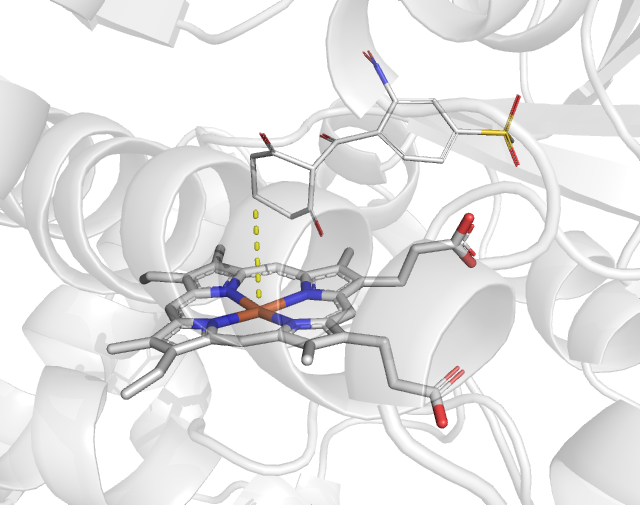
\includegraphics[width=\textwidth]{figs/score.png}
	\caption{\textbf{\label{score}} Distance of the mesotrione $C_5$ to the heme iron visualised from a docking pose, constituting the term $d_i$}
\end{figure}
\par
\subsubsection{Virtual Directed Evolution Experiment 1}
Initially, the virtual directed evolution program in this state was with no constraint on Hamming distance relative to the wild-type for 20 generations with a population size of 100 over the course of two days \textbf{(experiment 1)}. 

\begin{figure}[H]
	\caption{\label{experiment-1} \ref{violin} Violin plot showing the gradual improvement in fitness distributions \textbf{equation \ref{eqn}} over generations of virtual directed evolution in \textbf{experiment 1}. Fitness is a rescaled from the ordinal score such that 1 is the best score and 0 the worst.  \ref{hamming} Fitness increase with $n$ mutations relative to the wild type. \ref{tsne} t-Stochastic Neighbour Embedding (t-SNE) plot of the fitness landscape mapped in \textbf{experiment 1}, where clusters of points represent mutants with similar chemical properties in their active sites and color is mapped to a rescaled score where 1 is the best and 0 is the worst.}
	\begin{subfigure}{0.49\linewidth} 
		\caption{\label{violin}}
	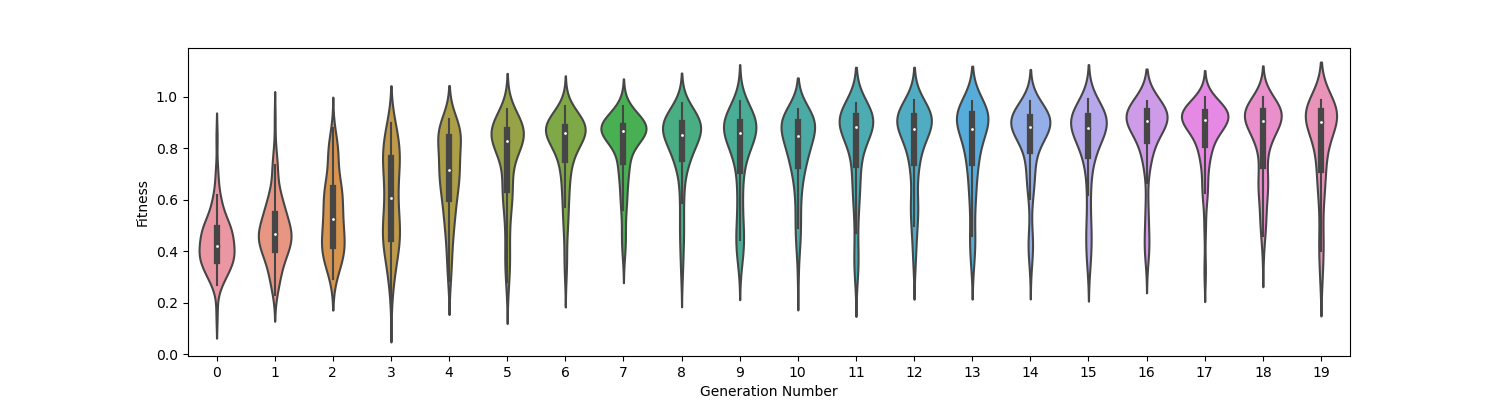
\includegraphics[width=\textwidth]{figs/molcv-fitness-violin.png}
	\end{subfigure}
	\begin{subfigure}{0.49\linewidth}
		\caption{\label{hamming}}
		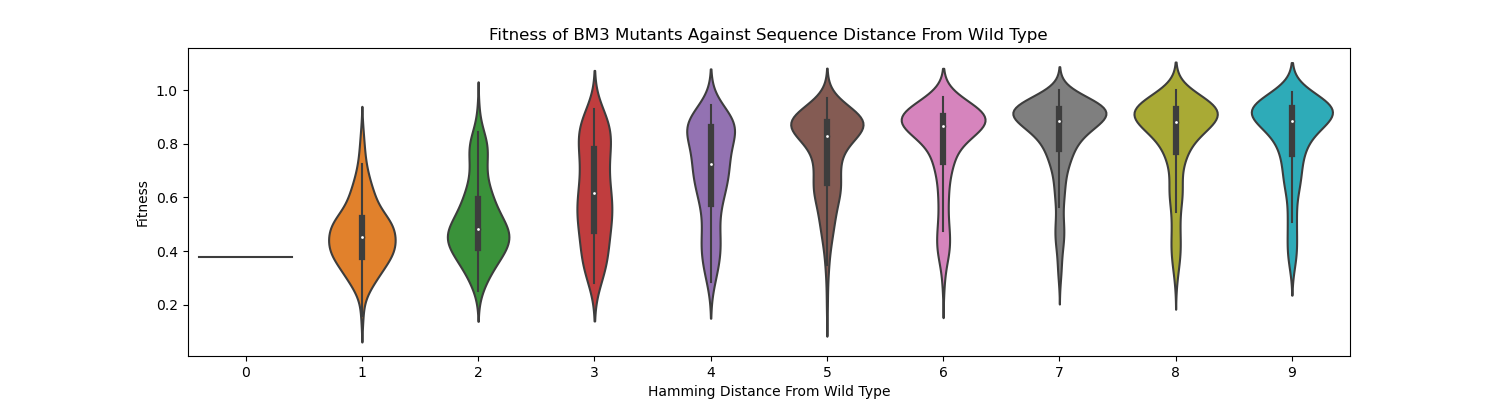
\includegraphics[width=\textwidth]{figs/hamming-violin.png}
	\end{subfigure}
	\begin{subfigure}{0.9\linewidth}
		\caption{\label{tsne}}
	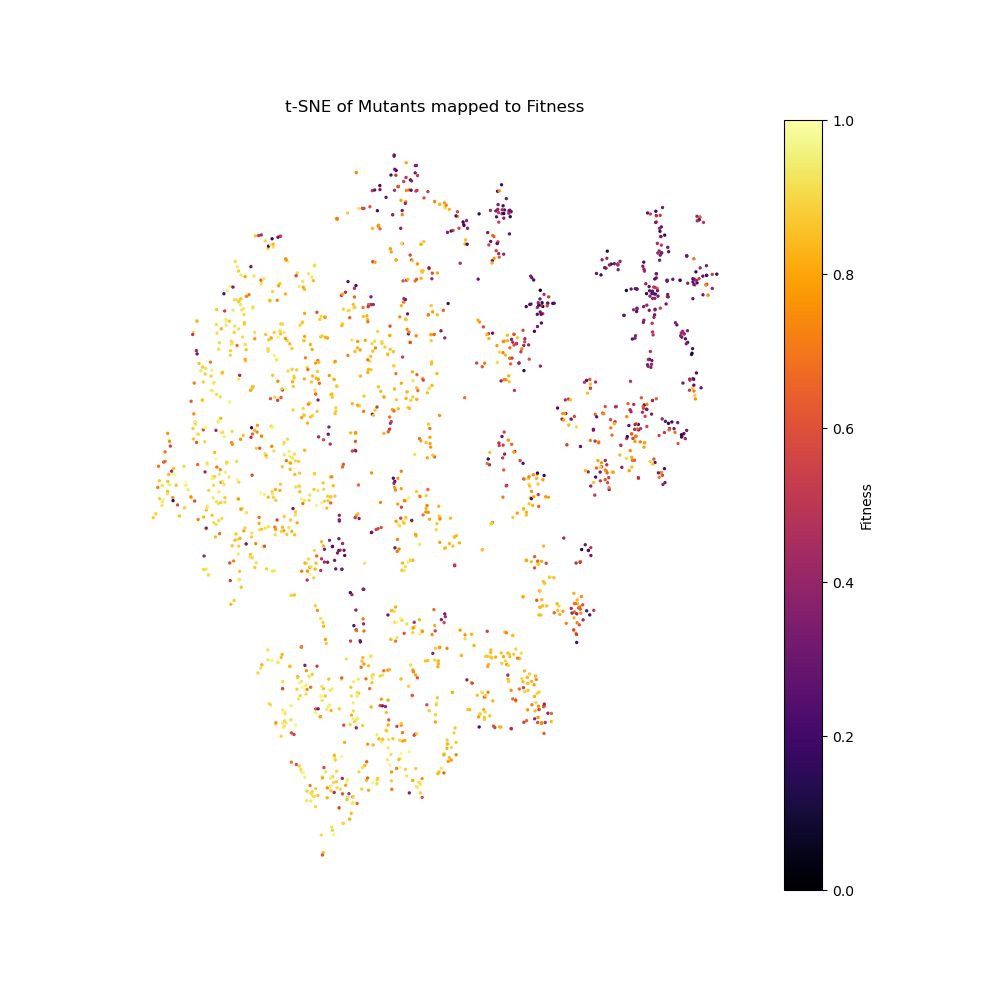
\includegraphics[width=\textwidth]{figs/moclv-tsne.png}
	\end{subfigure}
\end{figure}
\par


\begin{figure}[H] \label{dock}
	\caption{\label{dock} Comparison of the wild type and the best performing mutant from the virtual directed evolution \textbf{experiment 1} docked with mesotrione}
	\begin{subfigure}{0.49\textwidth}
		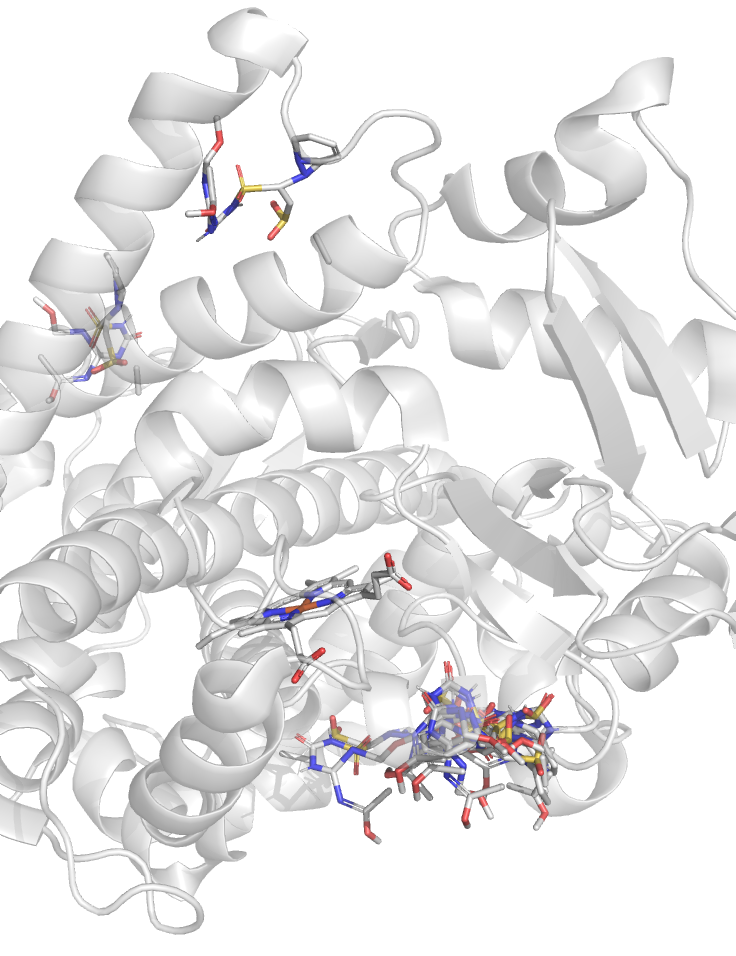
\includegraphics[width=\linewidth]{figs/wt-mesotrione.png}
		\caption{BM3 wild type docked with mesotrione, where no poses are in the binding site}
	\end{subfigure}
	\begin{subfigure}{0.49\textwidth}
		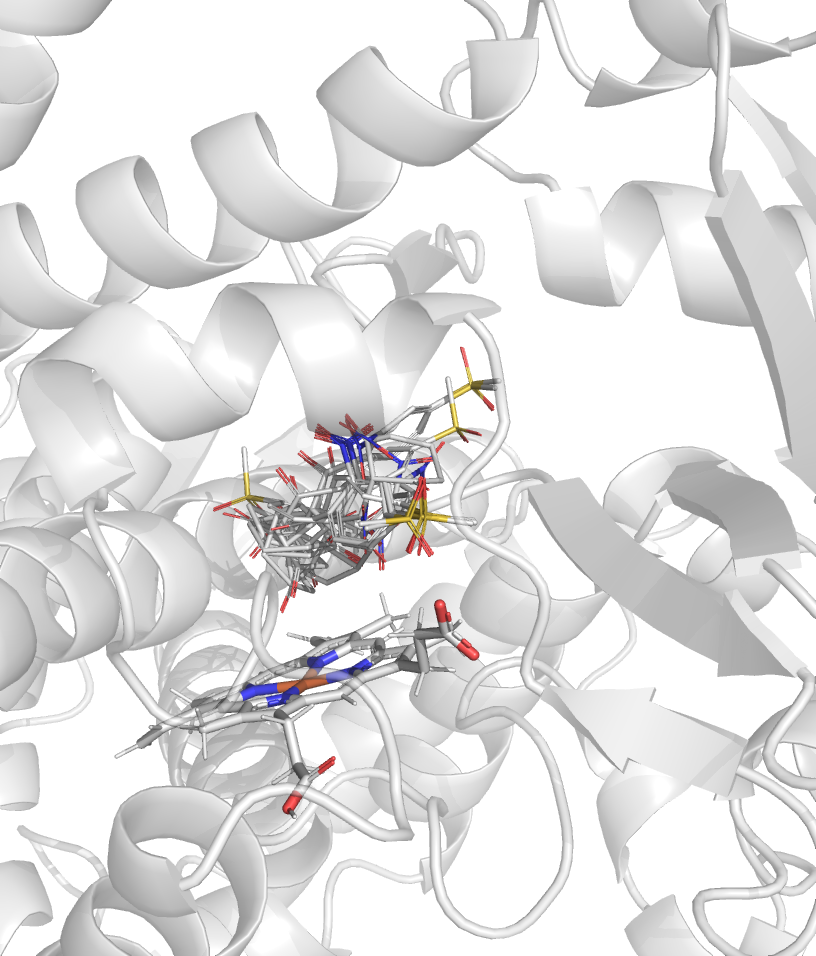
\includegraphics[width=\linewidth]{figs/best-mesotrione-RSKGVFAFK.png}
		\caption{The best performing mutant (47R/49S/51K/75G/78V/82F/87A/88F/94K)
docked with mesotrione where all poses are in the active site and aligned with $C_5$ towards the heme iron. All poses bound with $\Delta G$ <6 kcal/mol}
	\end{subfigure}
\end{figure}
%\par 
The virtual directed evolution experiment was a success in as far as it delivered several BM3 mutants with very favourable binding towards mesotrione, however a notable issue with the \textbf{experiment 1} is that I have accidentally constrained mutation sites to a small subset of active site amino acids. This issue was trivial to rectify and was patched.  The mutations listed are still suitable for some analyses and developing the subsequent synthesis programs (section \ref{mxn evo}). Subsequent experiments have indicated that most beneficial mutations occur in this small subset anyway.
\par
Despite the issue, several mutants with favourable binding towards mesotrione were identified. \textbf{Figure \ref{dock}} shows poses of bound mesotrione in the best performing mutant compared to the wild-type. This data was used to develop \texttt{mxn}, a primer design program (section \ref{mxn evo}).
\par

\subsubsection{Virtual Directed Evolution Experiment 2}

The second set of virtual directed evolution experiments address the issue of predicted mutants being many mutations away from existing templates, which results in a synthesis with a large number of steps. To address this, a permutation of equation \ref{eqn} was developed that takes into account the mutation (Hamming) distance between the mutant and the wild type:

\begin{equation}\label{eqn2}
	score = \frac{1}{n}\Sigma _{N} \Delta G_{i} \times d_{i} \times \frac{H}{k}
\end{equation}

where $H$ is the Hamming distance between the query sequence and the existing BM3 wild type and $k$ is an adjustment factor to be tweaked near run time.
Hamming distance is accounted for to minimize the number of site-directed mutagenesis steps whilst making and testing the mutants. 
\par
By using this score function, mutants are penalized for having a large mutation distance from the wild type, which results in mutants with favourable mesotrione binding whilst often being within five mutations from the wild type.
\par 
To increase the local sequence space explored, the survival rate of each pool was increased from $\frac{1}{4}$ to $\frac{1}{2}$ and the experiment was run with a population size of 80 for 50 generations.
\par
Again, this run identified many mutants with favourable binding towards mesotrione with the mean distance $d$ between the $C_5$ carbon and the heme iron being within 7 \AA - which positions mesotrione favourably. $K$ was 10, favouring desirable binding over $H$. This resulted in a large number of sequences with a large $H$ being evaluated. \textbf{Figure \ref{exp2-description}} shows summary statistics for the experiment. 
\par
The larger sample size allowed the identification of a Pareto optimization front, where two optimization objectives conflict. In this case, the Hamming distance from the wild type $H$ and $d$ are in conflict (\textbf{figure \ref{pareto}}), creating a trade off between $H$ and $d$. 
\par 
\textbf{Figure \ref{exp2-best-mutant}} shows the best scoring mutant for this experiment, 75A/87T/255D/290C, where $d$ is 7.7 \AA, a mean $\Delta G$ of -8.0 kcal / mol and $H = 4 $. The most favourable mutant by $d$ was 75A/87P/88S/94C/138M/142H/ 205R/226W/252Y/255W/260R/263S (\textbf{figure \ref{exp2-best-binding}}) where $d = 5.5$ \AA, $\Delta G = -7.7$ kcal / mol and $H$ was 12, which would be difficult to synthesize. The experiment identified some issues with the docking box parameters, which included an area outside the active site below the heme, introducing interference with the score metric (\textbf{figure \ref{exp2-issue}}), which is trivial to resolve in future runs.

\newgeometry{vmargin=1.5cm}
\begin{figure}[H]
	\caption{\label{experiment2} Summary statistics of virtual directed evolution experiment 2}
	\begin{subfigure}{0.9\textwidth}
		\caption{\label{exp2-description} Subplots showing kernel density estimates for the distributions of the score (equation \ref{eqn2}), mesotrione binding affinities, mean distances $d$ between $C_5$ carbons and the heme iron, and the Hamming distance $H$ of each mutant relative to the wild type.}
		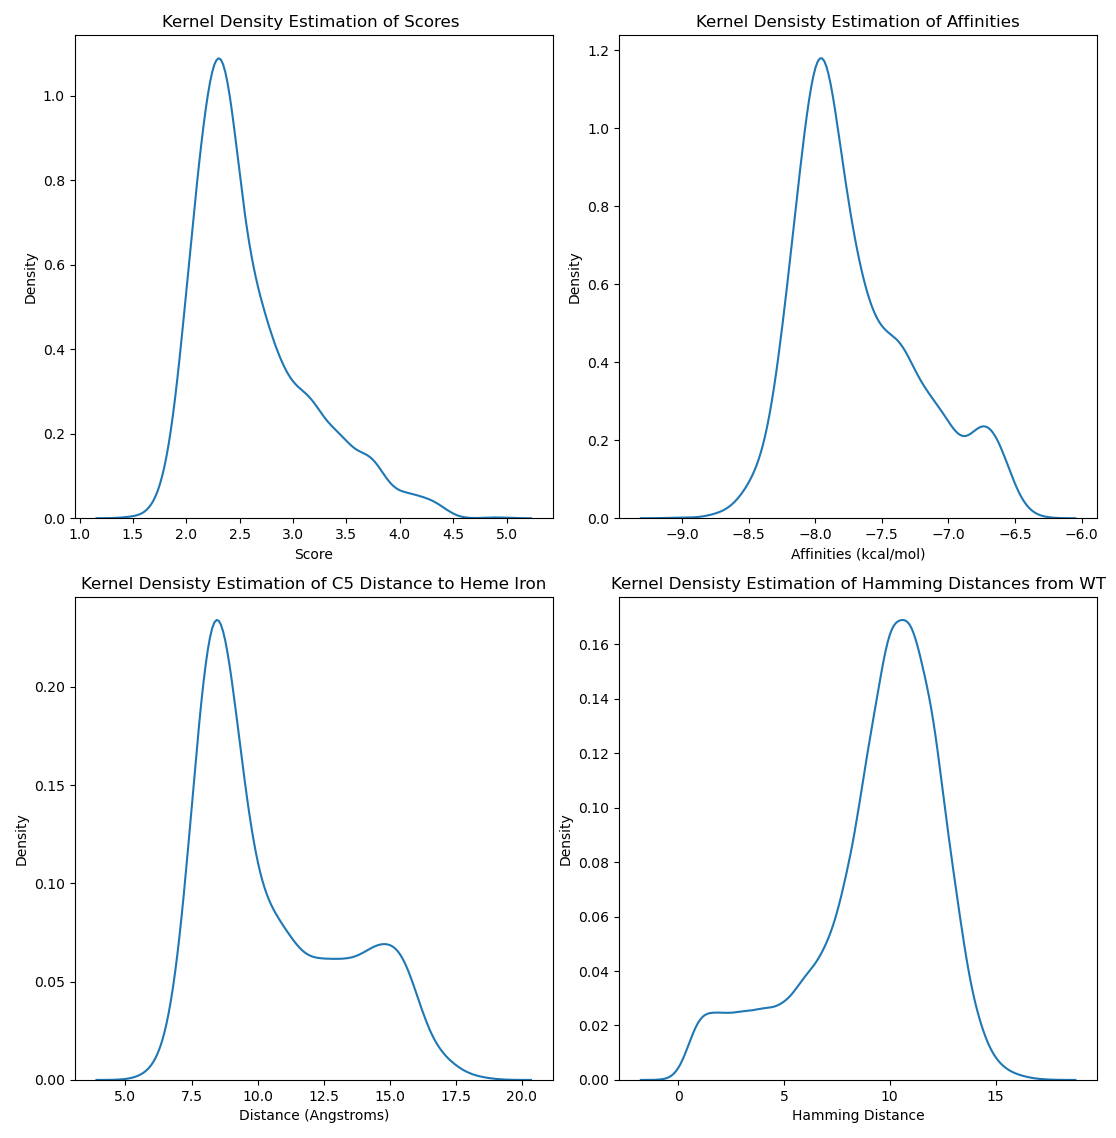
\includegraphics[width=\linewidth]{figs/uvwsl-description.png}
	\end{subfigure}
	\begin{subfigure}{0.49\textwidth}
		\caption{\label{pareto} The Pareto optimization front showing the conflict between $d$ and $H$ where each point is one mutant, color mapped to binding affinity (kcal / mol)}
		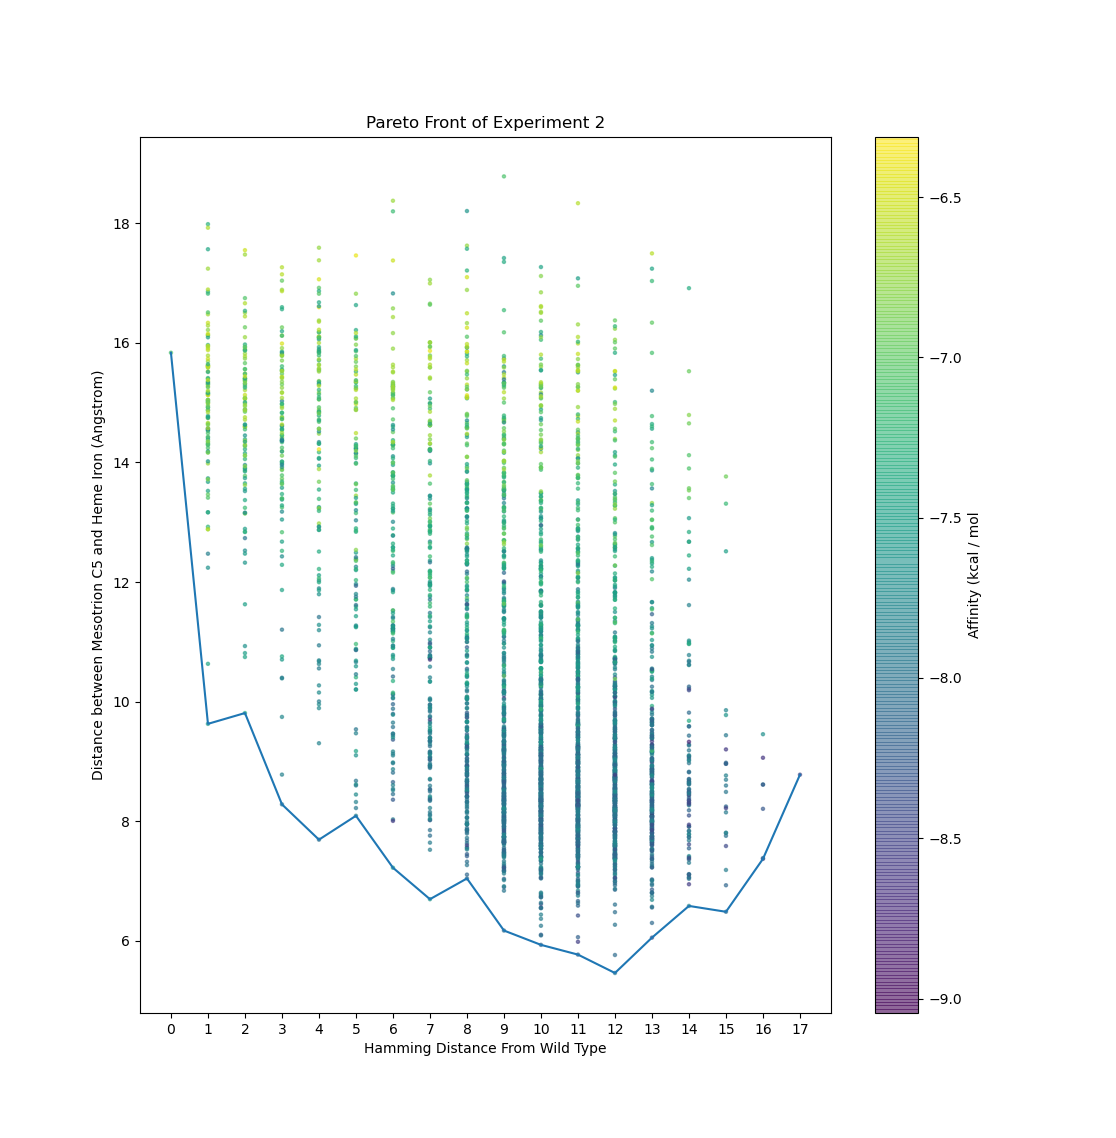
\includegraphics[width=\linewidth]{figs/uvwsl-pareto.png}
	\end{subfigure}
	\begin{subfigure}{0.49\textwidth}
		\caption{\label{exp2-tsne} T-SNE of mutants tested in experiment 2, color mapped to mean mesotrione $C_5$ distance to the heme iron. $d < 7$ is favourable.}
		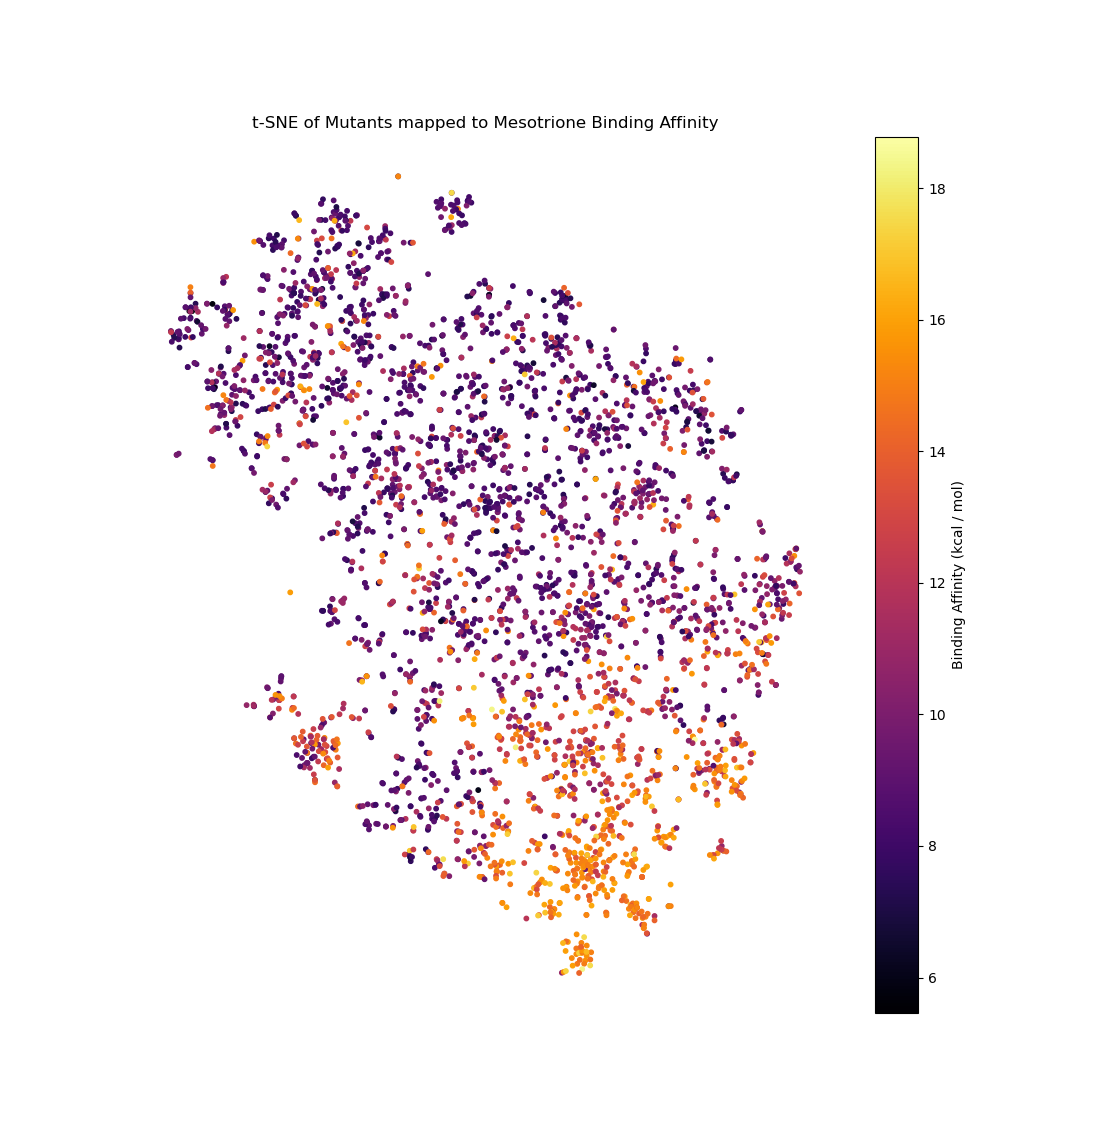
\includegraphics[width=\linewidth]{figs/uvwsl-ft-tsne.png}
	\end{subfigure}
\end{figure}
\restoregeometry

\begin{figure}[H]
	\begin{subfigure}{0.49\textwidth}
		\caption{\label{exp2-best-mutant} The best performing mutant in experiment 2 by measure of equation \ref{eqn2} 75A/87T/255D/290C}
		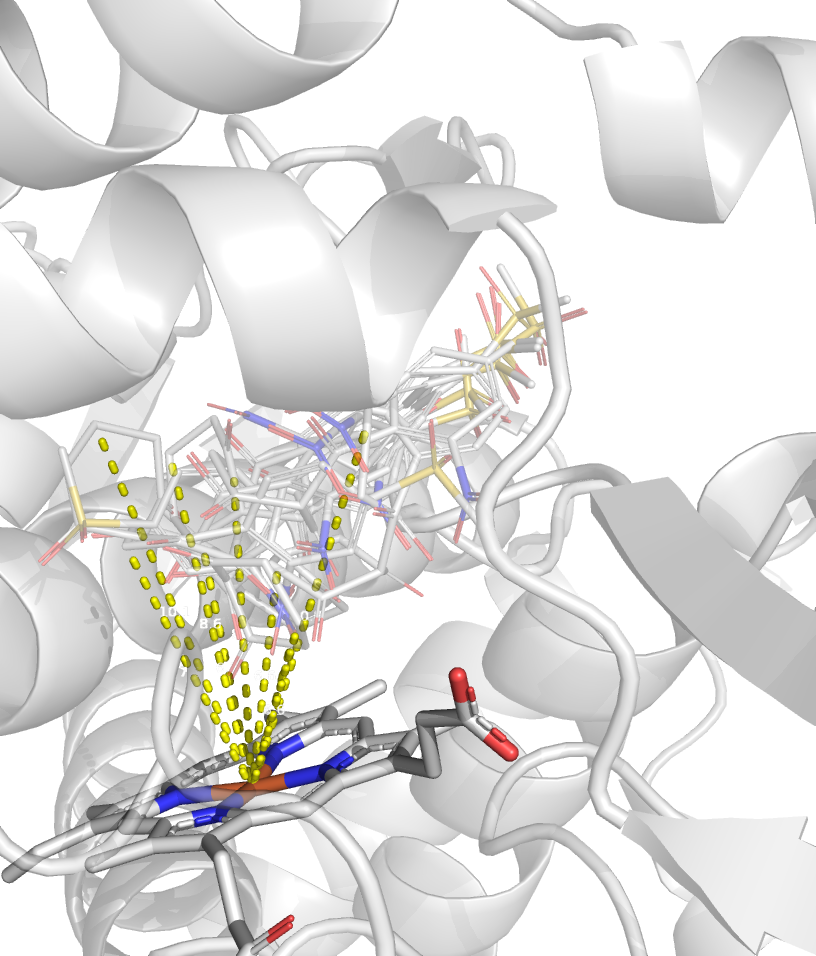
\includegraphics[width=\linewidth]{figs/exp2-best-dock.png}
	\end{subfigure}
	\begin{subfigure}{0.49\textwidth}
		\caption{\label{exp2-best-binding} The most favourable binding conformation by $d$ in experiment 2 75A/87P/88S/94C/138M/142H/ 205R/226W/252Y/255W/260R/263S}
		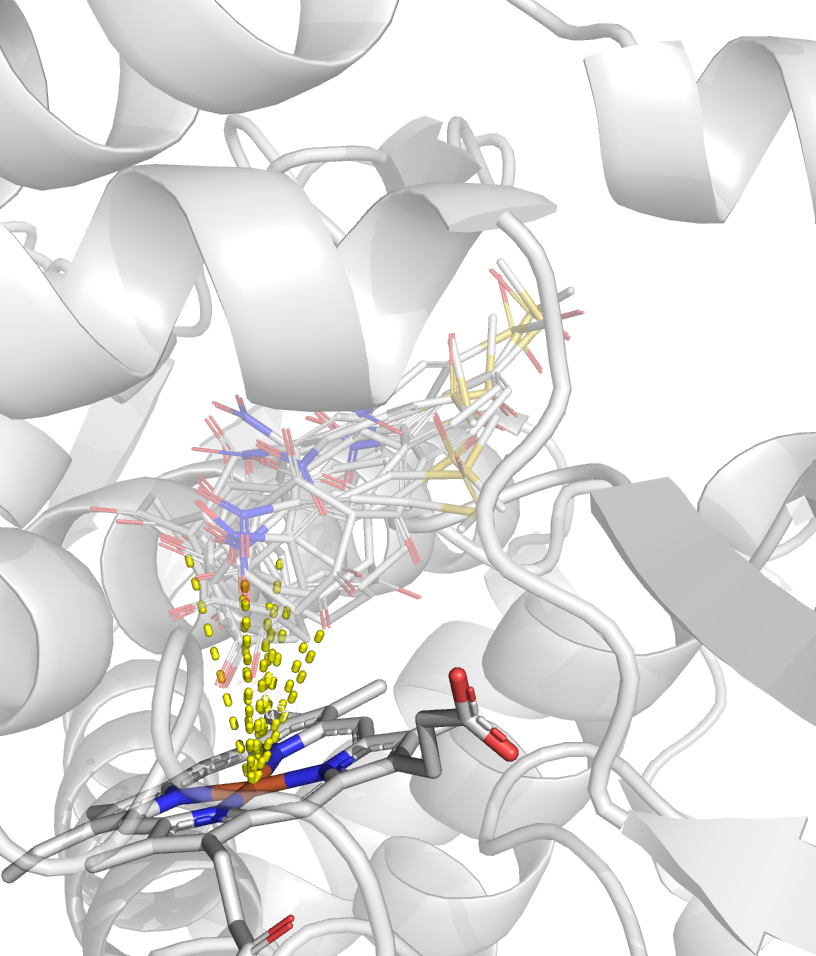
\includegraphics[width=\linewidth]{figs/exp2-best-aff-dock.png}
	\end{subfigure}
	\begin{subfigure}{0.49\textwidth}
		\caption{\label{exp2-issue} An issue identified in experiment 2 where the docking box includes areas not in the active site, interfering with the score function.}
		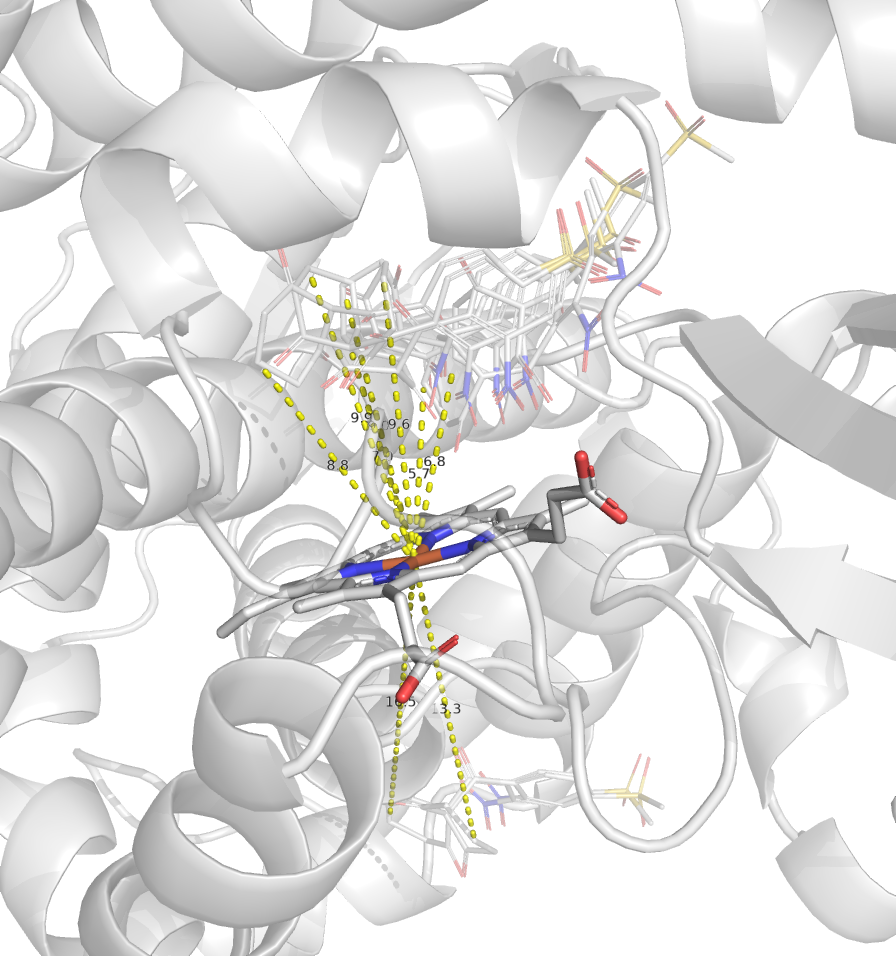
\includegraphics[width=\linewidth]{figs/exp2-issue.png}
	\end{subfigure}
\end{figure}

\subsubsection{Primer Design with \texttt{mxn}} \label{mxn evo}
The BM3 variants selected for testing in the lab should be a diverse set of the fittest mutants. Few mutants close to the wild type (by Hamming distance) are particularly fit (\textbf{figure \ref{hamming}}), therefore it is important that the mutation strategy used can efficiently produce a diverse set with the fewest possible steps. The strategy used here involves \textbf{1)} identifying the shortest mutation path to all targeted mutants and \textbf{2)} automated primer design. % synthesis plan

\par
With the preliminary data from experiment 1, the selection technique and synthesis planning methods were developed. Eight mutants were sampled from the fittest 30\% of the total population screened using Max Min sampling - a technique which maximises the minimum distance between each member of a set. % diversity sampling
\textbf{Table \ref{mutant table}} shows an example of a diversity sampled set of the fittest mutants. % hamming distance

\begin{table}[h]
	\centering
\begin{tabular}{lllllllllr}
	\textbf{47} &   \textbf{51} &   \textbf{75} &   \textbf{82} & \textbf{87} &   \textbf{88} &   \textbf{94} &   \textbf{49} &   \textbf{78} &   \textbf{Fitness} \\
\hline
   P &    H &    G &    F &  A &    F &    T &  - &  - &  0.971868 \\
   F &    N &  - &  - &  H &  - &  - &    F &    A &  0.728075 \\
   S &    M &    N &    Y &  G &    P &    D &    S &    P &  0.736979 \\
   E &  - &    P &    D &  T &    H &  - &    M &  - &  0.845709 \\
   K &  - &    G &  - &  C &    Y &    L &    W &    L &  0.853135 \\
 - &    V &    P &    G &  G &  - &    S &  - &    I &  0.874266 \\
   A &    N &    G &    K &  G &    W &    I &    P &    E &  0.855940 \\
   P &    R &    D &    M &  P &    K &    M &    A &    L &  0.825515 \\
\end{tabular}
	\caption{\label{mutant table} Example of diversity sampled mutants from the fittest 30\% of mutants in (\textbf{experiment 1}), columns correspond to mutation sites.}
\end{table}

\par
\texttt{mxn} is an automated primer design \textit{python} package developed for this work. \texttt{mxn} designs QuickChange-style primers for point mutations in a coding sequence compatible with the Agilent QuickChange cloning strategy. \texttt{mxn} uses nearest neighbor thermodynamics \cite{santalucia1998unified} and a DMSO correction factor \cite{von2001oligonucleotide} that gave a reasonable fit to primer $Tm$s calculated by the Agilent online calculator. Primers are extended $n$ and $m$ nucleotides up and downstream from the mutation site to satisfy an objective function that accounts for $Tm$ (and its closeness to 78°C), end GC content, hairpin $\Delta G$ and homodimer $\Delta G$ via simulated annealing \cite{kirkpatrick1983optimization}. %mxn
\par
The efficacy of primers designed with \texttt{mxn} are currently being tested (section \ref{mxn}).
\par
Given a list of mutations, it is straightforward to design all primers using \texttt{mxn}.

\subsubsection{Work to do}\label{vde-todo}
I am currently repeating experiment 2 with tweaks to $k$, the weighting of $\Delta G$ and $d$ and to the fraction of mutants that survive each generation, with the expectation that a higher survival rate coupled with more generations may give sufficient genetic drift for some very good mutations to emerge. Most immediately, I'm patching the issue identified in experiment 2 in the docking box size, which lead to confounding results.
\par
After a satisfactory virtual directed evolution run, I can diversity sample a selection of the fittest slice of the mutants as in table \ref{mutant table}. Given that there is a trade off between $H$ and $d$ for the mutants, I'm likely to get much better performing mutants with $H$ around 8, which can be achieved in two synthesis steps. The number of mutants I can make and test is limited by my grand budget.
\par
Following mutant design, primers will be designed \textit{en masse} using \texttt{mxn}. Primers designed using \texttt{mxn} are currently being tested for efficacy, however issues with sequencing and availability of material in the lab has set back this work. A reasonable date for DNA work to begin on this project is the week of the 24th of May. % re run and primers 
\par
Given that the template sequence is AT-rich and repetitive, DNA work can be challenging for some mutation sites. Therefore it would be prudent to order primers for more mutants than I plan to express in anticipation of a non-zero attrition rate of mutants. Since I want to test six-eight mutants, planning the DNA work for eight-ten may be sensible however, ``dangerous`` primers may be identified manually or automatically by their repetivity or their AT content. % dna work attrition rate
\par
The mutants will be designed from a full-length BM3 template, and will be expressed in 3 L batches - which allows eight mutants to be expressed with four 24 hour shaker slots. % expression 
These mutants can be purified over the course of one-two weeks and tested over a further one-two weeks. % purification
% testing
\par
Testing will comprise UV-Vis spectroscopy-based titrations with mesotrione to determine $K_d$ and NADPH consumption-based steady state kinetics to determine $K_M$ and $K_{cat}$. Indication of product formation with mesotrione using LCMS would be important to include too, but I have yet to set up a procedure for this.
\par
This represents the end state of this project. \textbf{Figure \ref{evoG}} shows a dependency graph of the remainder of this work. The Gannt chart in \ref{vde ganntt} shows the task queue for the remainder of this work.

%%%%%% graph fig %%%%%%%%%%%%%
\begin{figure}[H]
	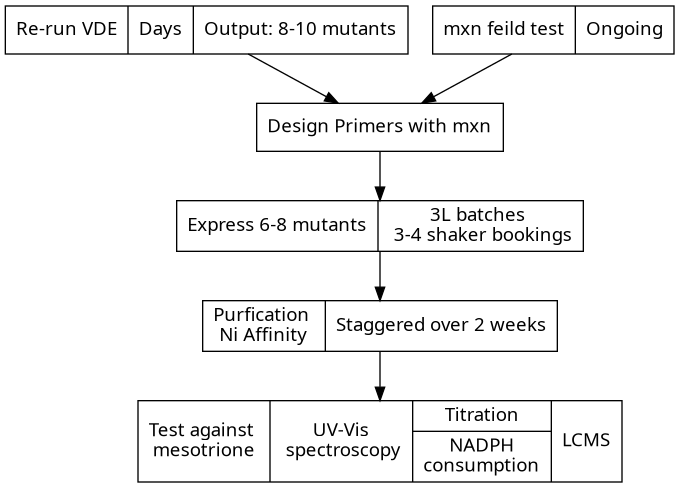
\includegraphics[width=0.9\textwidth]{figs/evoG.png}
	\caption{\label{evoG} Dependency graph of remainder of the virtual directed evolution project}
\end{figure}

%%%%%%%%%%%%%%%%%%% ganntt chart
\newgeometry{vmargin=1cm}
\begin{landscape}
	\subsubsection{Gantt Chart}\label{vde gantt}
	\centering
\begin{ganttchart}[time slot format=isodate, x unit = 1.9mm, vgrid, hgrid]{2021-05-17}{2021-09-18}{week}
	\gantttitlecalendar{month = name, week=3} \\
	\ganttbar{VDE}{2021-05-17}{2021-05-25} \\
	\ganttbar{Primer Design}{2021-05-25}{2021-05-26} \\
	\ganttbar{Primer Shipping}{2021-05-26}{2021-06-03} \\
	\ganttbar{DNA work}{2021-06-03}{2021-06-17} \\
	\ganttbar{Expression}{2021-06-11}{2021-06-25} \\
	\ganttbar{Purification}{2021-06-18}{2021-07-03} \\
	\ganttbar{Validation}{2021-07-03}{2021-07-10} \\
\end{ganttchart}
\end{landscape}
\restoregeometry

\section{AI-Based Design}
This enzyme engineering technique aims to  use a relatively sophisticated machine learning model to estimate the $K_d$ between a given P450 sequence and a small molecule SMILES. Using a set herbicide as an input SMILES, many sequences can be queried using any sequence optimization algorithm with predictions being made very quickly by the model.
\par 
The model is trained on screening data generated as part of this work, where several notably promiscuous mutants of BM3 are screened for $K_d$ against many compounds using an assay developed for this work. A pre-training phase on data mined from KEGG is essential for success and has been demonstrated to be critical for effective learning on small datasets in similar, enzyme engineering domains \cite{biswas2021low}.

\subsection{Work to Date}
\subsubsection{384 well Plate Binding Assay and Screening}
A high throughput assay for measuring $K_d$ between a P450 and a small molecule was developed for this work, including the software necessary for design and analysis of the experiments. The assay is a 384 well plate assay that uses a Labcyte Echo acoustic liquid handler to add precise (to 2.5 nl) amounts of ligand in DMSO to the plate. The current format employed for screening uses eight concentrations of each ligand, accommodating 48 compounds per plate. 96 compounds per screening round is practical.
\par
The assay is a 384 well plate-based analog of traditional UV-Vis spectroscopy-based titrations of P450s used to determine $K_d$ between enzyme and compound. On binding to a substrate, a P450 gives a measurable shift in its UV-Vis absorbance; $K_d$ is determined by fitting a Michaelis Menten curve to the response at different concentrations. If the compound itself has a UV-Vis absorbance profile that interferes with with the P450 absorbance profile, then a dual-beam spectrometer is used where for each increment in substrate concentration, the same increment is made in a second cuvette. The trace from the second cuvette is subtracted from the sample to correct for the compound absorbance.
\par
The 384 well plate assay works in the same way, where each compound (in DMSO) is dispensed in 8 concentrations and topped up to a constant volume with DMSO (5\% v/v) using a \textit{Labcyte Echo} - an acoustic liquid handling robot. 5 \% DMSO is tolerated by BM3, and must be kept constant because it can induce a mild response that would otherwise be a false positive. Assay volume is 30 µl, which is the minimum volume that gives a reliable signal. Low assay volume saves not only protein, but compound too. Protein is added to plates at 10 µM ofter compounds and DMSO have been dispensed, which gives a good signal. Protein is buffered in 100 mM KPi at pH 7, which is a standard buffer for BM3. The buffer additionally contains 0.1 \% Bovine Serum Albumen (BSA) to improve stability. The buffer is thoroughly de-gassed prior to use to avoid bubble formation. Plates are centrifuged before reading to remove bubbles and ensure that well contents is seated at the bottom of the well. The assay remains stable at 4 °C for over an hour, however this freezes the DMSO which interferes with the assay. Therefore the assay should be kept at room temperature. Previous tests with the wild type indicate that signal is still good after over an hour.
\par
A second plate containing only compounds in buffers is also created for correction of compound absorbance. On measurement, absorbance for each well is taken from 250 - 800 nm, which takes 9 minutes per plate. 
\par
The software developed for this assay comprise a \textit{python} package for design of the experiment and generation of picklists for the \textit{Echo} - \texttt{echo} and a \textit{python} package for analysis of the plate data - \texttt{plates}.
\par
Analysis of plate data using \texttt{plates} follows procedures used when analysing UV-Vis spectroscopy data:
\begin{enumerate}
	\item (optionally) Gaussian smoothing of traces
	\item zero at 800 nm
	\item subtract control traces
	\item measure absolute changes in absorbance at 420 and 390 nm
	\item fit Michaelis Menten 
\end{enumerate}
\par 
\textbf{Figure \ref{goodplates}} shows three examples of screening results gathered so far where results have been of a good standard.
\par
\begin{centering}
\begin{figure}[H]
	\centering
	\caption{\label{goodplates} Pranlukast, Trimethoprim and Altretamine(Hexalen) screened against A82F/F87V, A82F/F87V and A82F respectively.}
	\begin{subfigure}{\linewidth}
		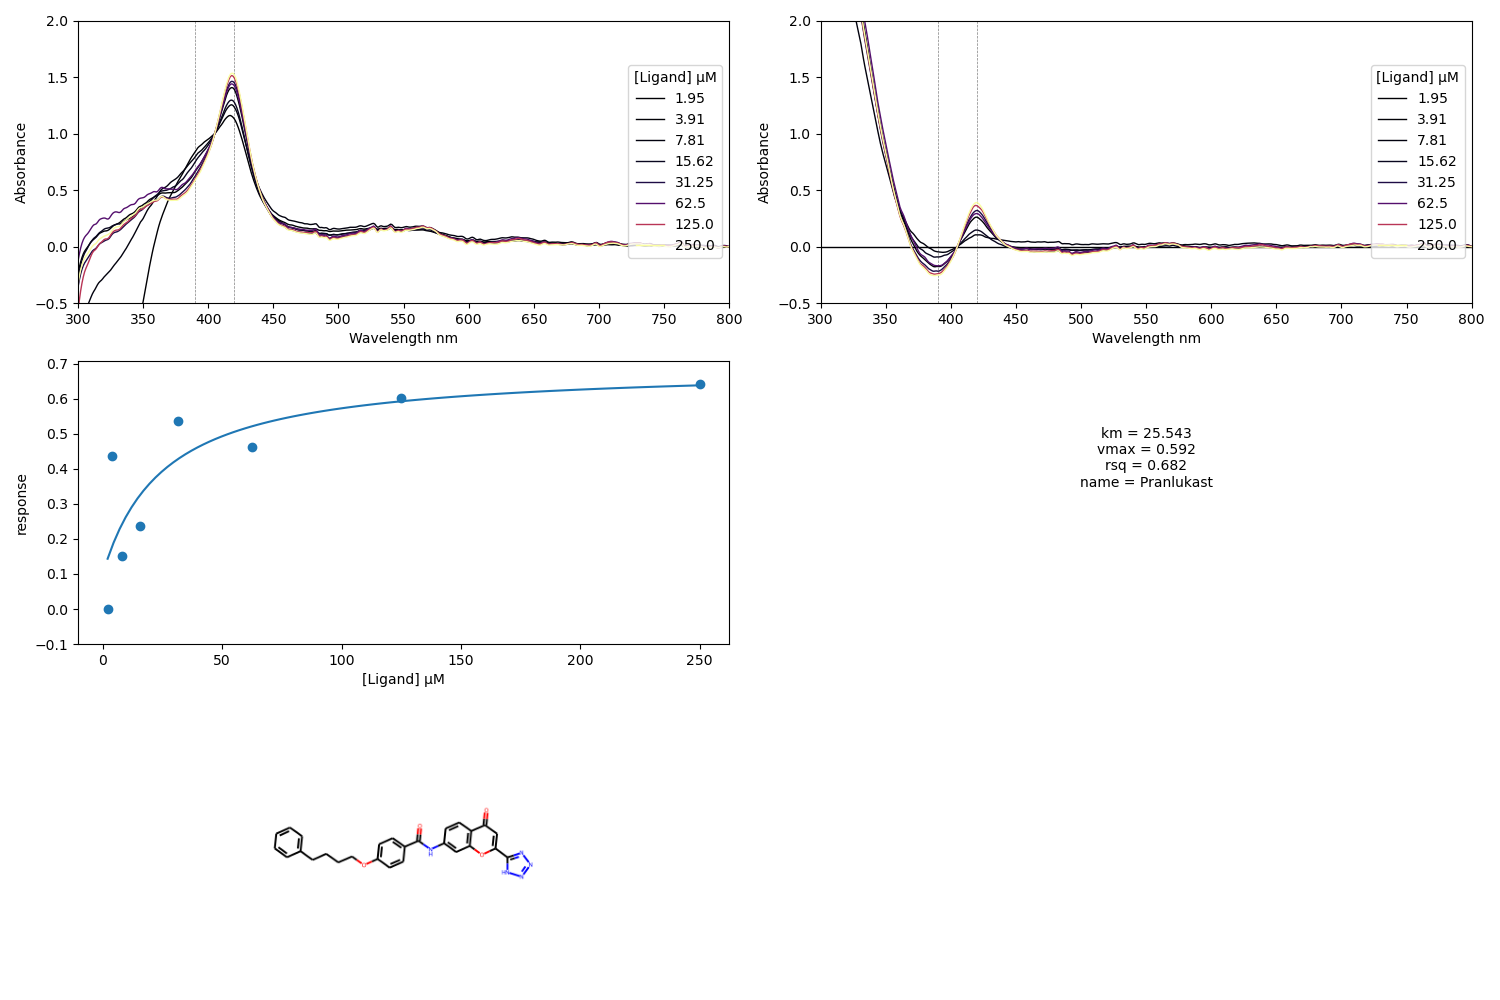
\includegraphics[width=0.7\textwidth]{figs/Pranlukast.png}
	\end{subfigure}
	\begin{subfigure}{\linewidth}
		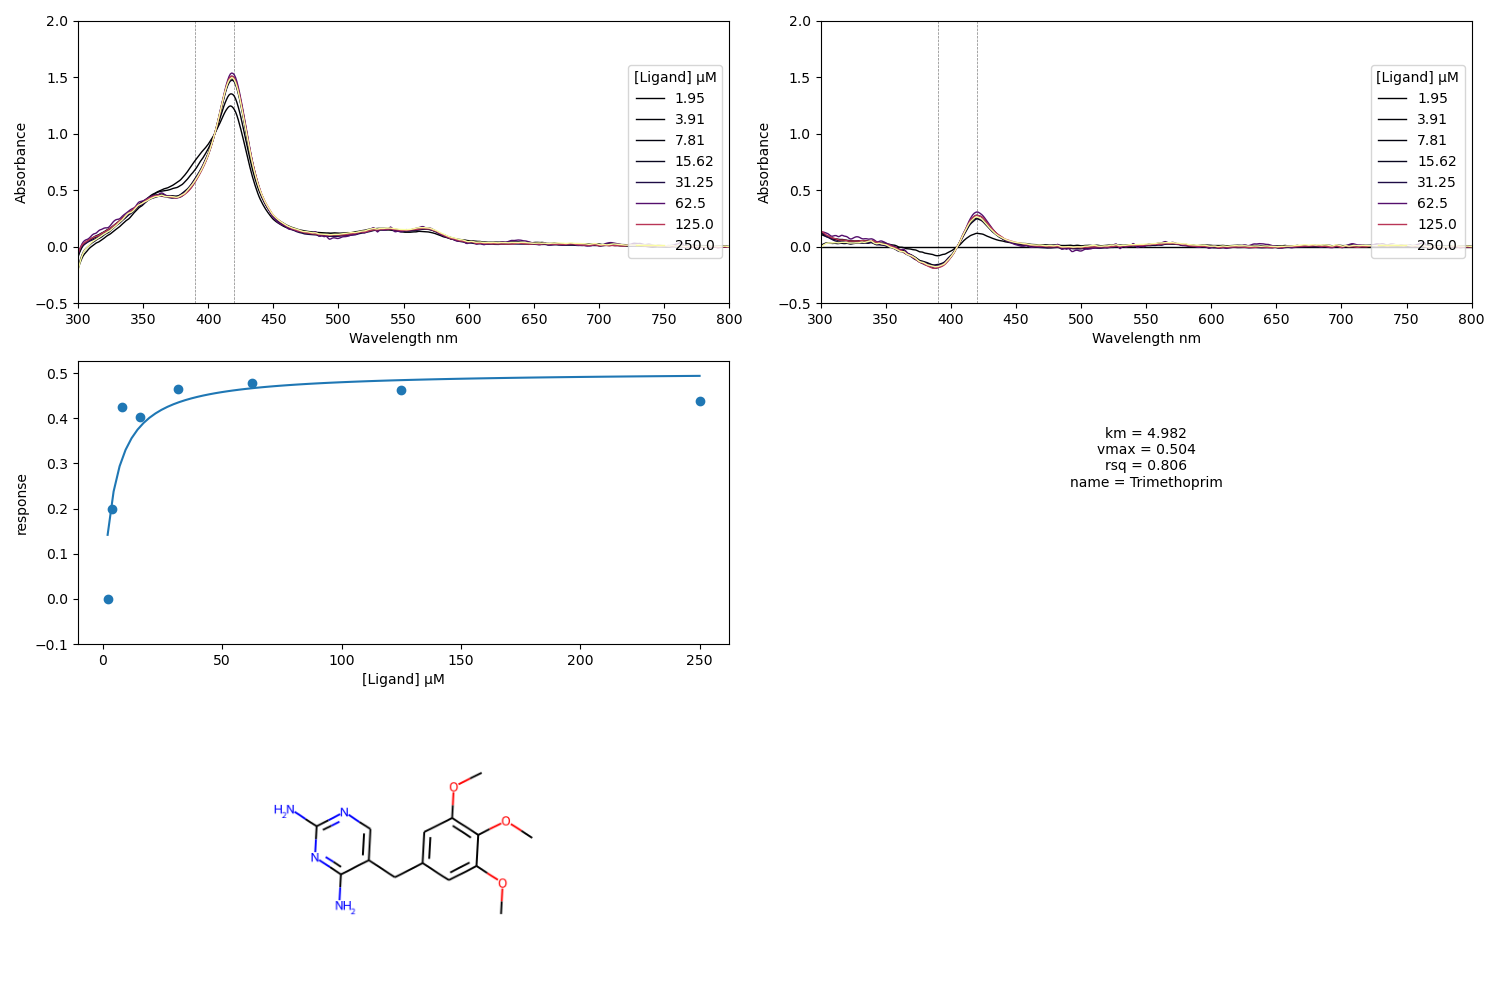
\includegraphics[width=0.7\textwidth]{figs/Trimethoprim.png}
	\end{subfigure}
	\begin{subfigure}{\linewidth}
		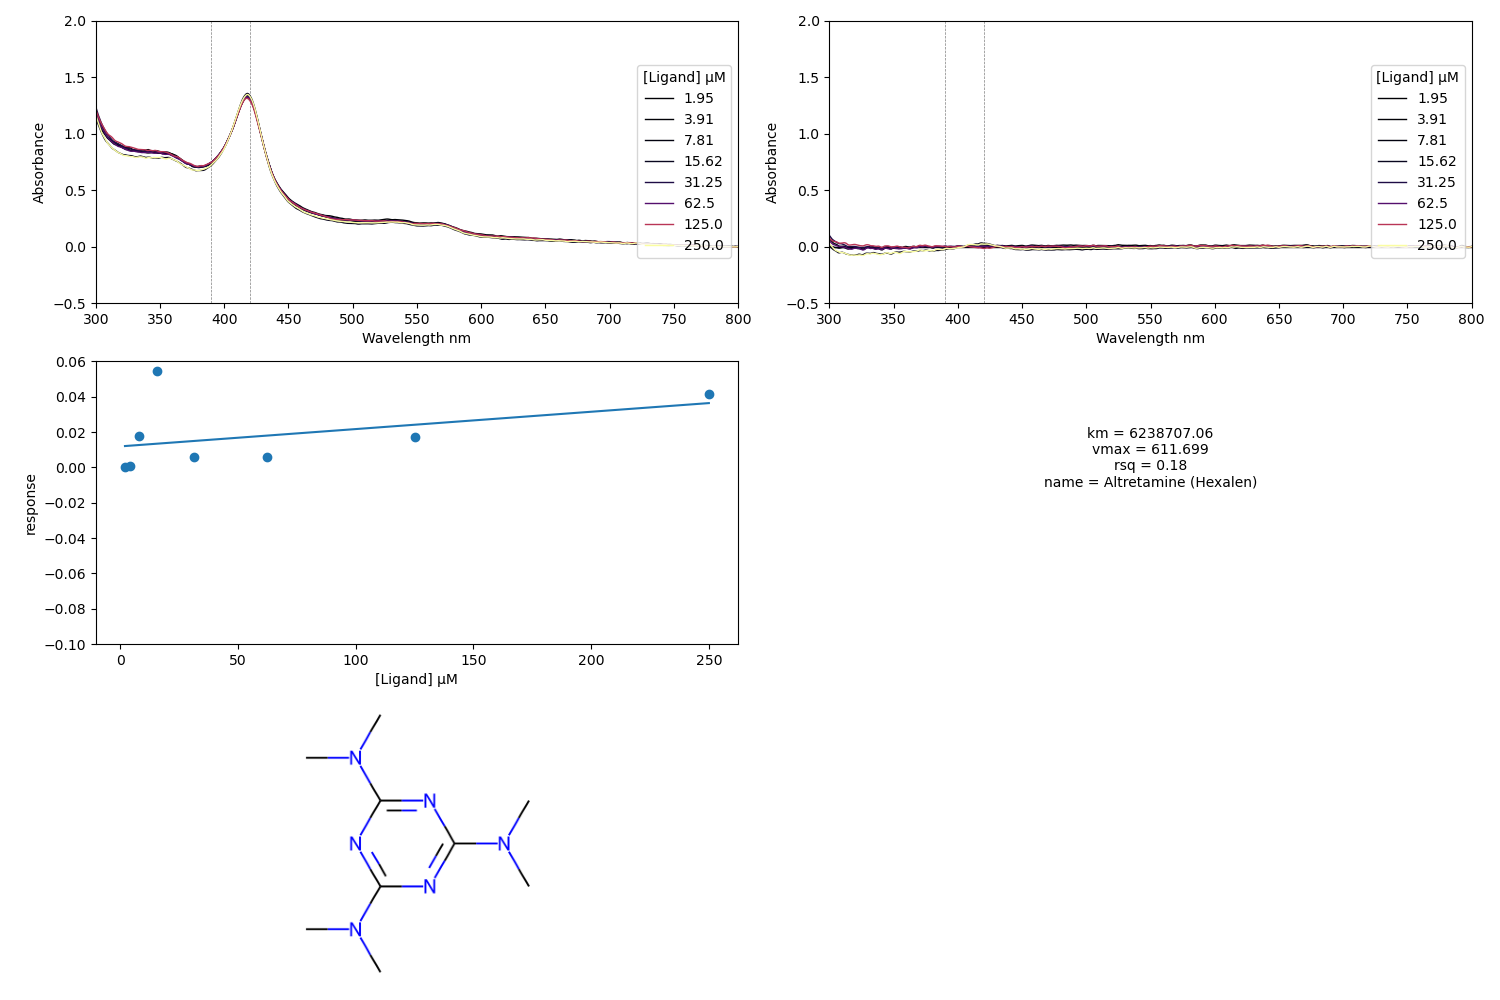
\includegraphics[width=0.7\textwidth]{figs/Altretamine(Hexalen).png}
	\end{subfigure}
\end{figure}
\end{centering}
\par
\textbf{Figure \ref{plates}} shows three example binding assay reports for BM3 A82F/F87V with different substrates which are below standard and need debugging. \ref{15} shows a relatively successful experiment with one anomaly whilst \ref{31} shows weak to no binding with the substrate with an unusual trace at 3.91 µM of substrate where the usual Soret peak at 420 nm is split into two at 400 and 420 nm, possibly a result of compound absorbance normalization. Strange errors like this are not unusual. \ref{32} shows a non-binding substrate with a Rayleigh scattering anomaly at 15.62 µM of substrate, likely either the result of protein precipitation or a bubble in the well. % example report
\par
Many of the compounds screened here absorb in the 280 nm region, which may be due to light scattering of solids in solution. A possible cause is chemical precipitation, which I have limited control over; another is that DMSO ice may be forming when I hold my plates at 4°C between runs on the plate reader which is below the freezing temperature of DMSO (19°C). This can be remedied by keeping the plates at room temperature. Stable BM3 variants should withstand this, whilst with less stable variants it is a necessary risk.  % todo
\par
I suspect that DMSO ice is a key issue in the messiness of some of the poorer signals, especially when the spectra of a protein-free control is subtracted, which may have different ammounts of DMSO ice-related scattering.
\par
Further development of \texttt{plates} will see anomaly detection and filtering of those anomalies and enabling identification of inhibitors via a type 2 Soret peak shift

\newgeometry{vmargin=2cm}
\begin{centering}
\begin{figure}[H]
	\centering
	\caption{\label{plates} Binding assay reports for three screening compounds against BM3 A82F/F87V made using \texttt{plates} with low quality results} %%%% todo - find out what chemicals
	\begin{subfigure}{0.7\textwidth}
		\caption{\label{15}}
		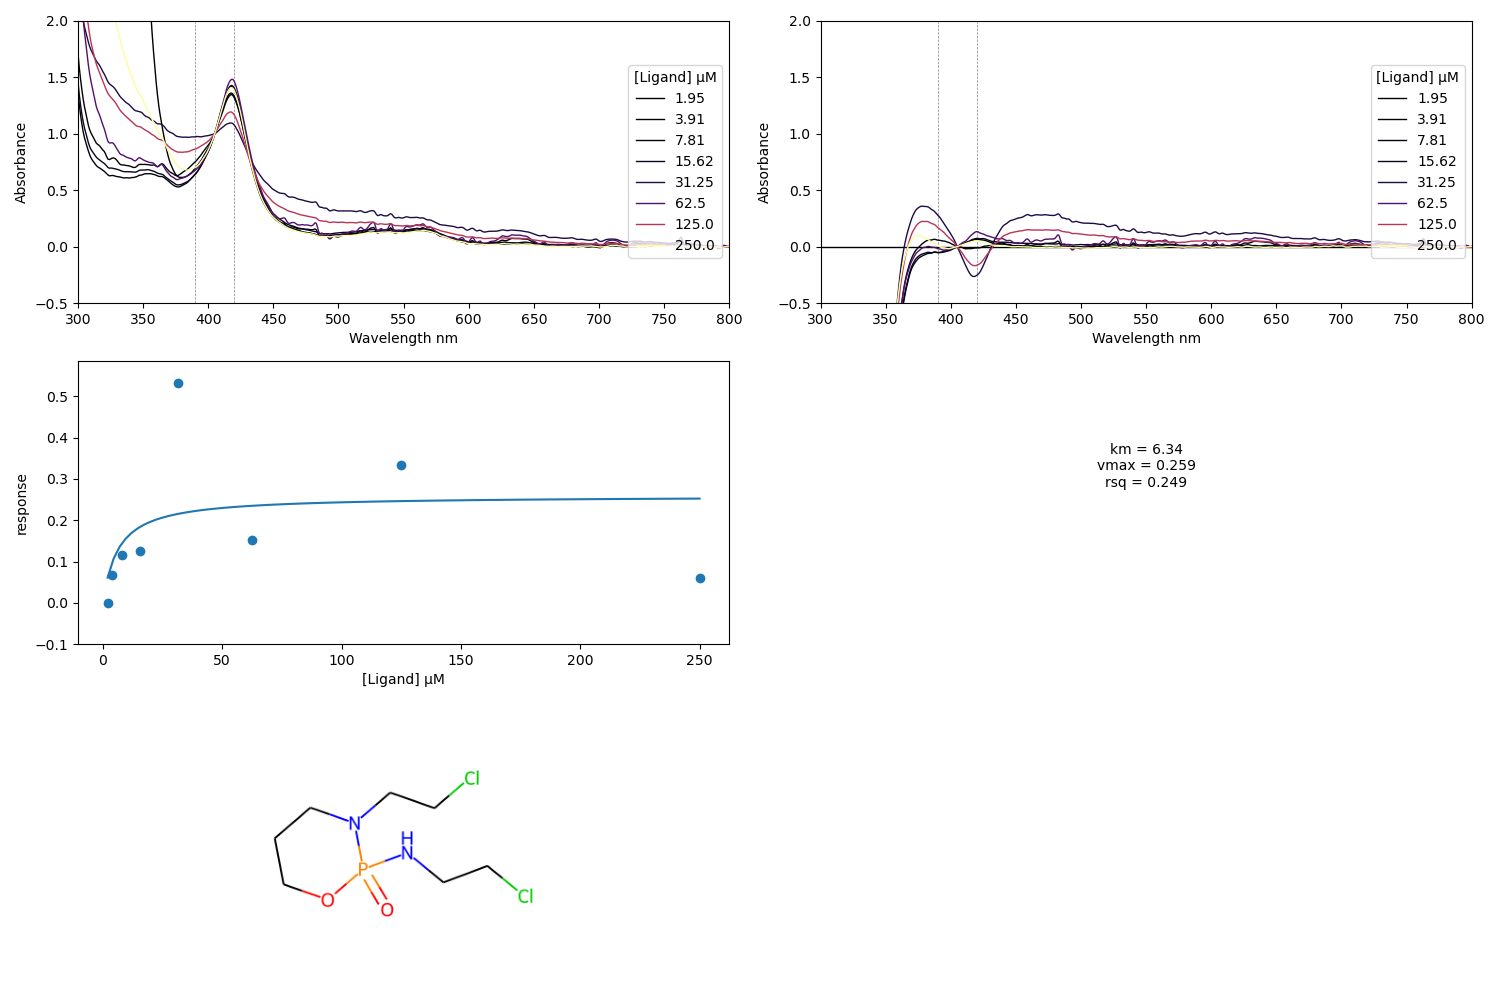
\includegraphics[width=\linewidth]{figs/15.png}
	\end{subfigure}
	\begin{subfigure}{0.7\textwidth}
		\caption{\label{31}}
		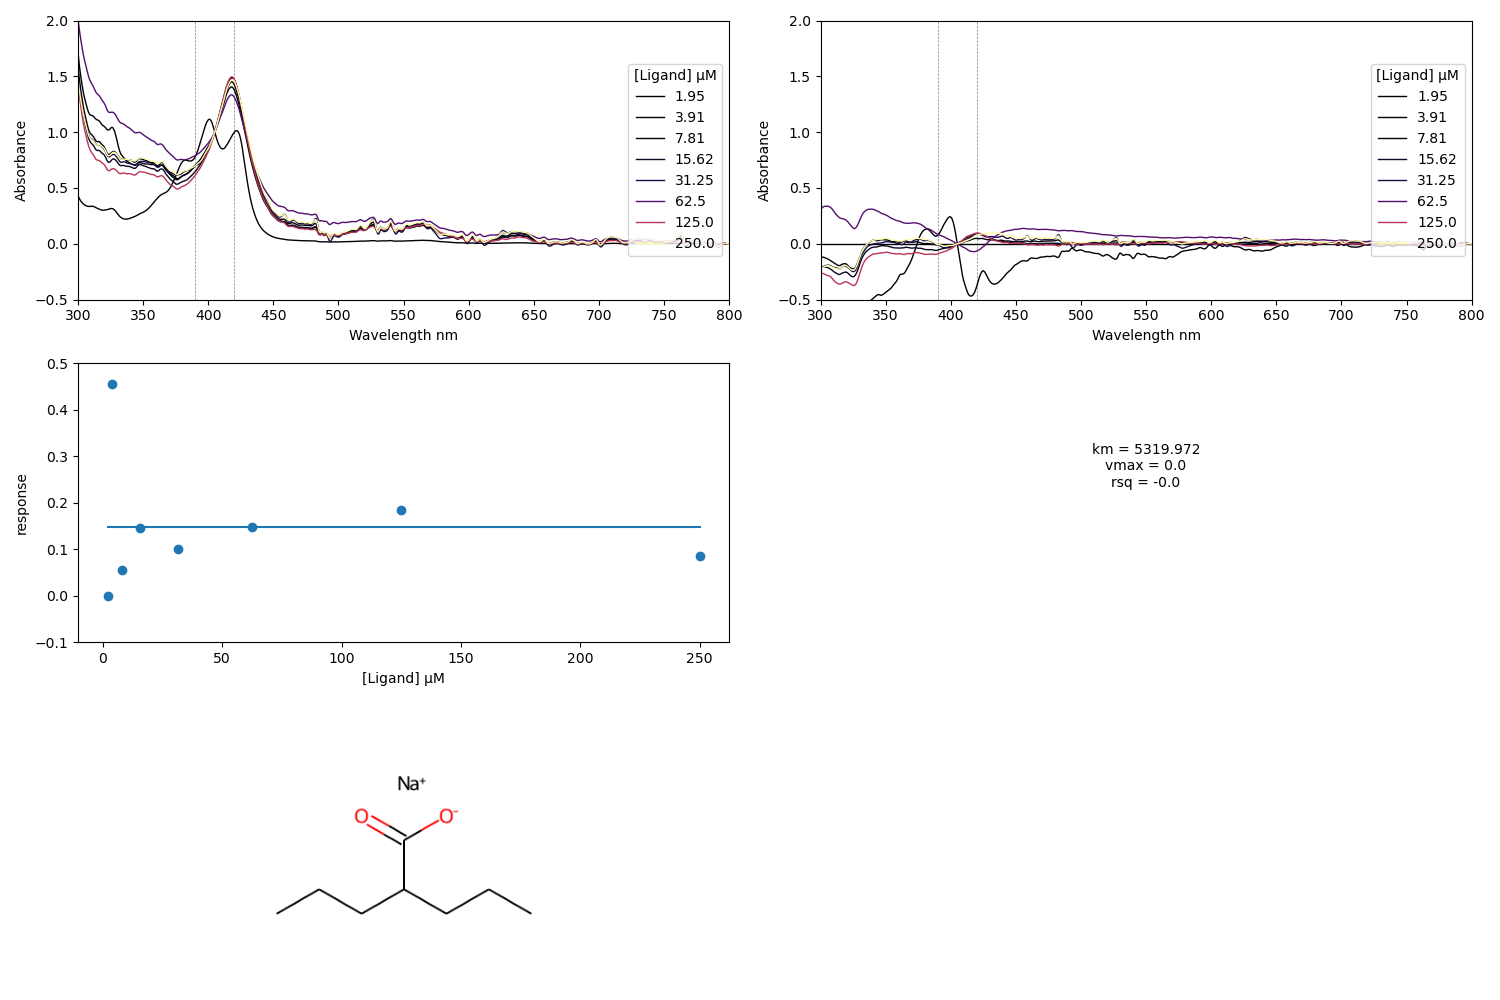
\includegraphics[width=\linewidth]{figs/31.png}
	\end{subfigure}
	\begin{subfigure}{0.7\textwidth}
		\caption{\label{32}}
		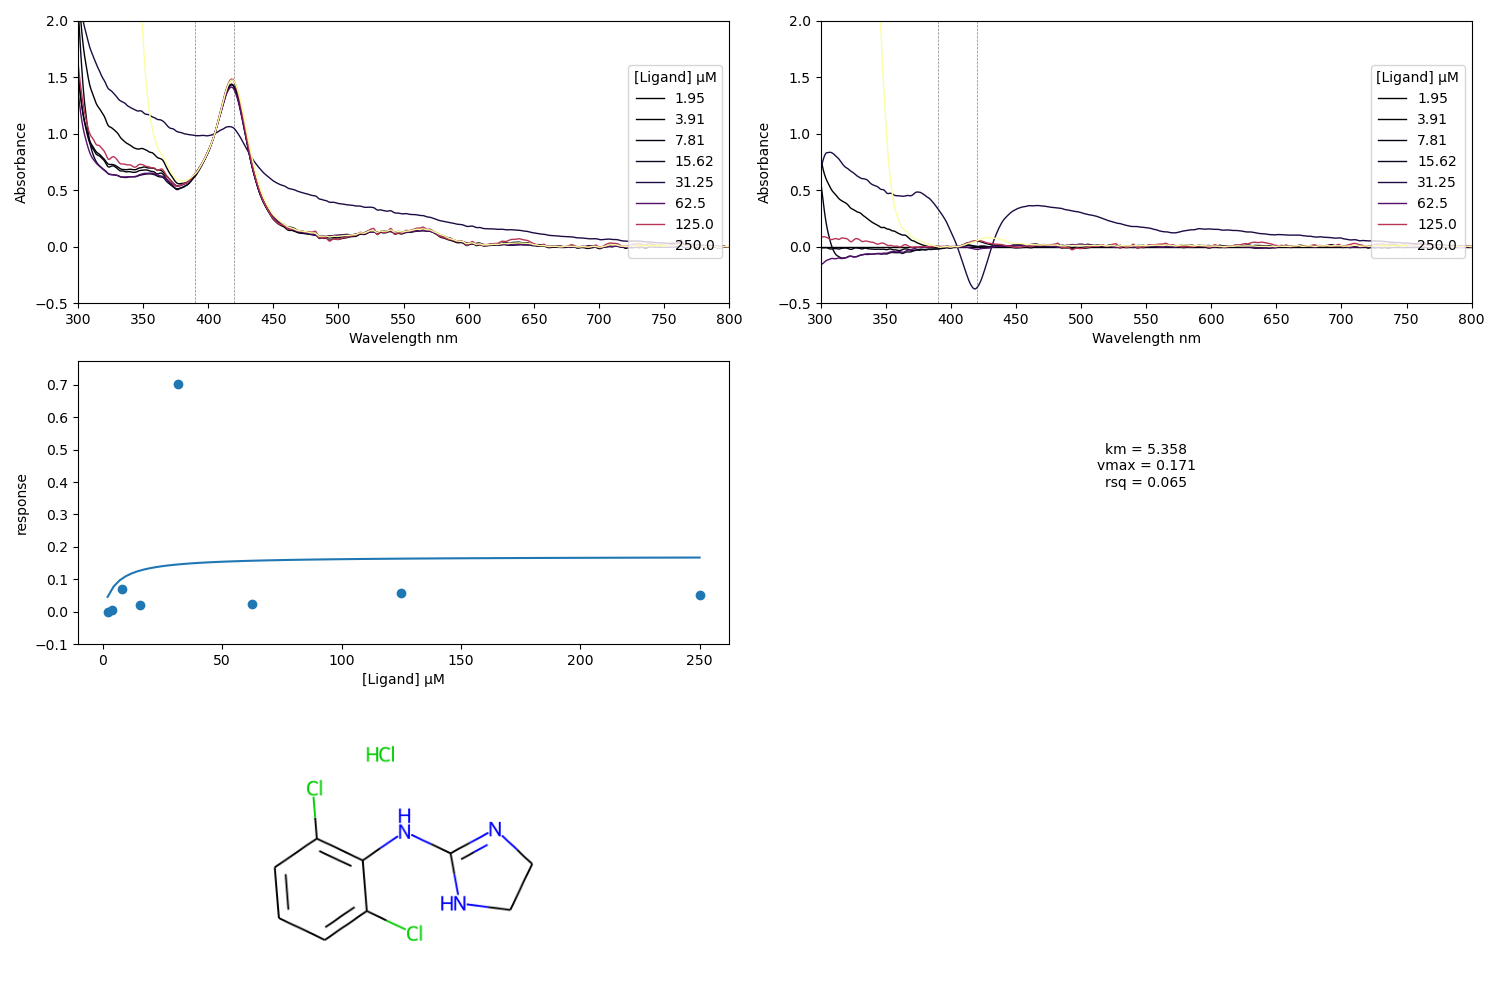
\includegraphics[width=\linewidth]{figs/32.png}
	\end{subfigure}
\end{figure}
\end{centering}
\restoregeometry

\par
So far, mutants have been screened for $K_d$ against the 96 compounds in batches of 3, where four hours is spent dispensing compounds and two-three hours is spent taking measurements. The two stages can be disconnected for practicality. The hours spent dispensing the compounds are periodically replacing one plate with another in the \textit{Echo} manually.
\par
Screening results so far are of reasonable quality and have helped the development of \texttt{plates}, the analysis \textit{python} package.   % results so far - example report 
\par
96 herbicide-like compounds have been screened against three BM3 variants so far (wild type, A82F, A82F/F87V). A further three mutants are pure and ready to be screened (K97C, A264E and A330P), following a recent failed attempt. 
\par
The herbicide-like compounds used here were from an existing in-house library of FDA-approved drugs, filtered from > 900 to around 300 using herbicide-likeness rules \cite{avram2014quantitative}. 96 structurally diverse compounds were selected from this subset using Maximum Minimum (MaxMin) diversity sampling \cite{porumbel2011simple}.
\par

\subsubsection{Screening Compound Selection}
I have implemented MaxMin to sample $n$ diverse herbicide-like compounds from a suppliers' database. The supplier, MolPort is an aggregator with over 2 million compounds available which can be shipped in any format. After filtering the library based on herbicide-likeness, MaxMin sampling is used to repeatedly sample diverse compound sets ($n$ = 96). 
MaxMin sampling is randomly seeded, so I sampled 100,000 diverse sets and used MolPort's database API to query price and shipping time estimates for all sets to find the cheapest and most readily available (\textbf{figure \ref{lib-cost}}). The cheapest sets are around 1,800 USD for 5mg of each compound - the minimum shipping size. I have been coordinating with my regional MolPort sales manager to arrange packing at 100 mM in DMSO and \textit{FluidX} vials, which are a very practical format for high throughput screening. I'll know what the handling cost is soon.
\par
I will need to adjust this program in two ways before ordering a selection: \textbf{1)} Update the compound database. \textbf{2)} Add an additional filter based on herbicide-likeness based on fingerprint Tanimoto similarity. This work is straightforward and shouldn't take long to implement.
\par
\textbf{Figure \ref{lib}} shows the cheapest library sampled using the re sampling technique. Given that the sampling space is so large, it would be prudent if I re sample again with an additional filter for herbicide likeness like molecular fingerprint Tanimoto similarity - a standard chemical similarity measurement. This should cut the space down to something more herbicide-like. 

\begin{figure}[H]
	\centering
	\caption{\label{lib-cost} Price estimate distributions of 100,000 proposed compound libraries with $n = 96$}
	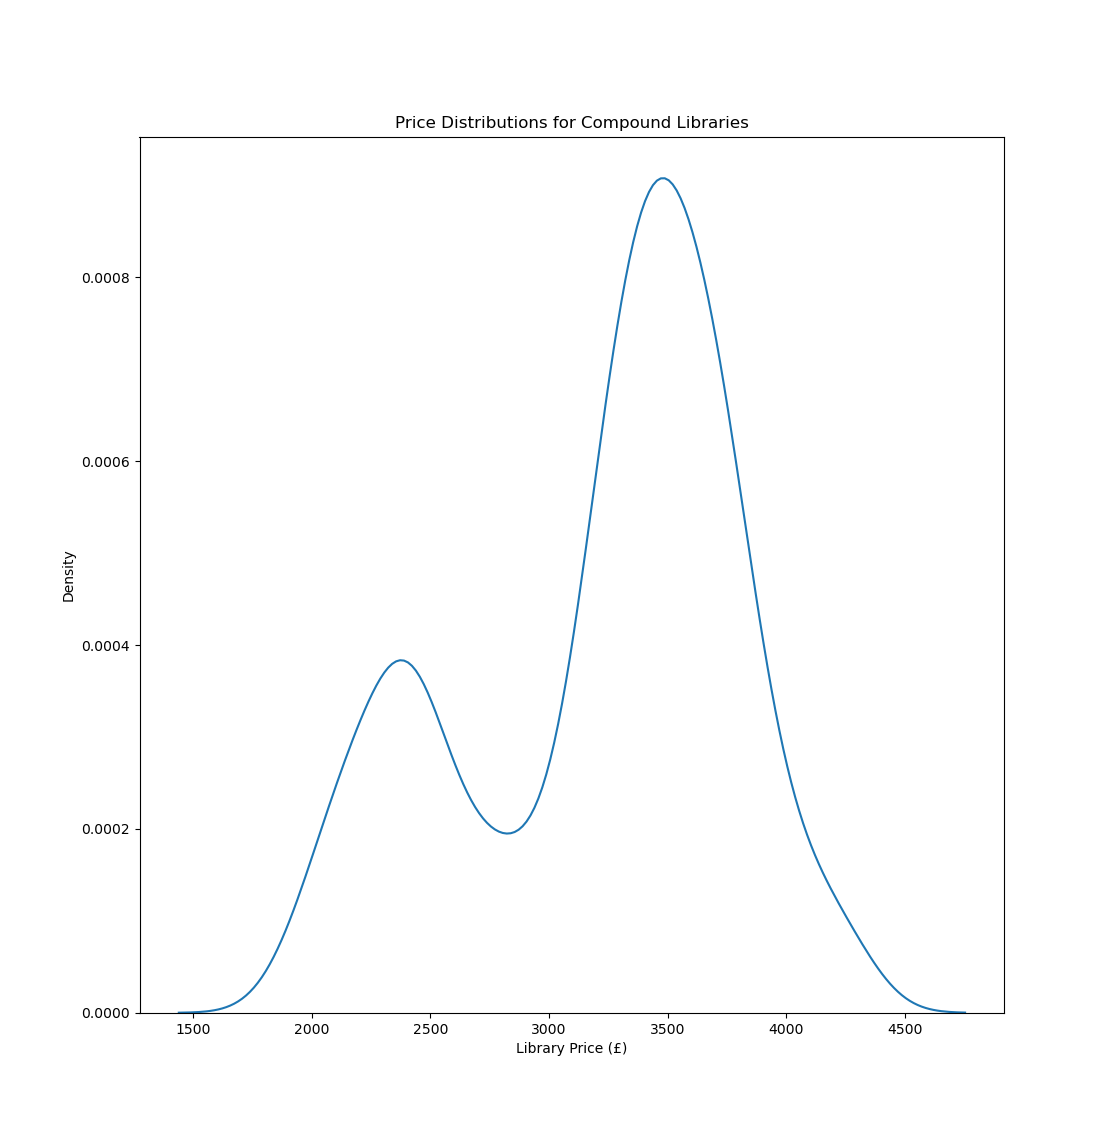
\includegraphics[width=0.5\textwidth]{figs/lib_costs.png}
\end{figure}

\begin{figure}[t]
	\caption{\label{lib} The cheapest library generated using the re sampling technique, an estimated cost of 1877 USD - excluding handling and shipping. }
	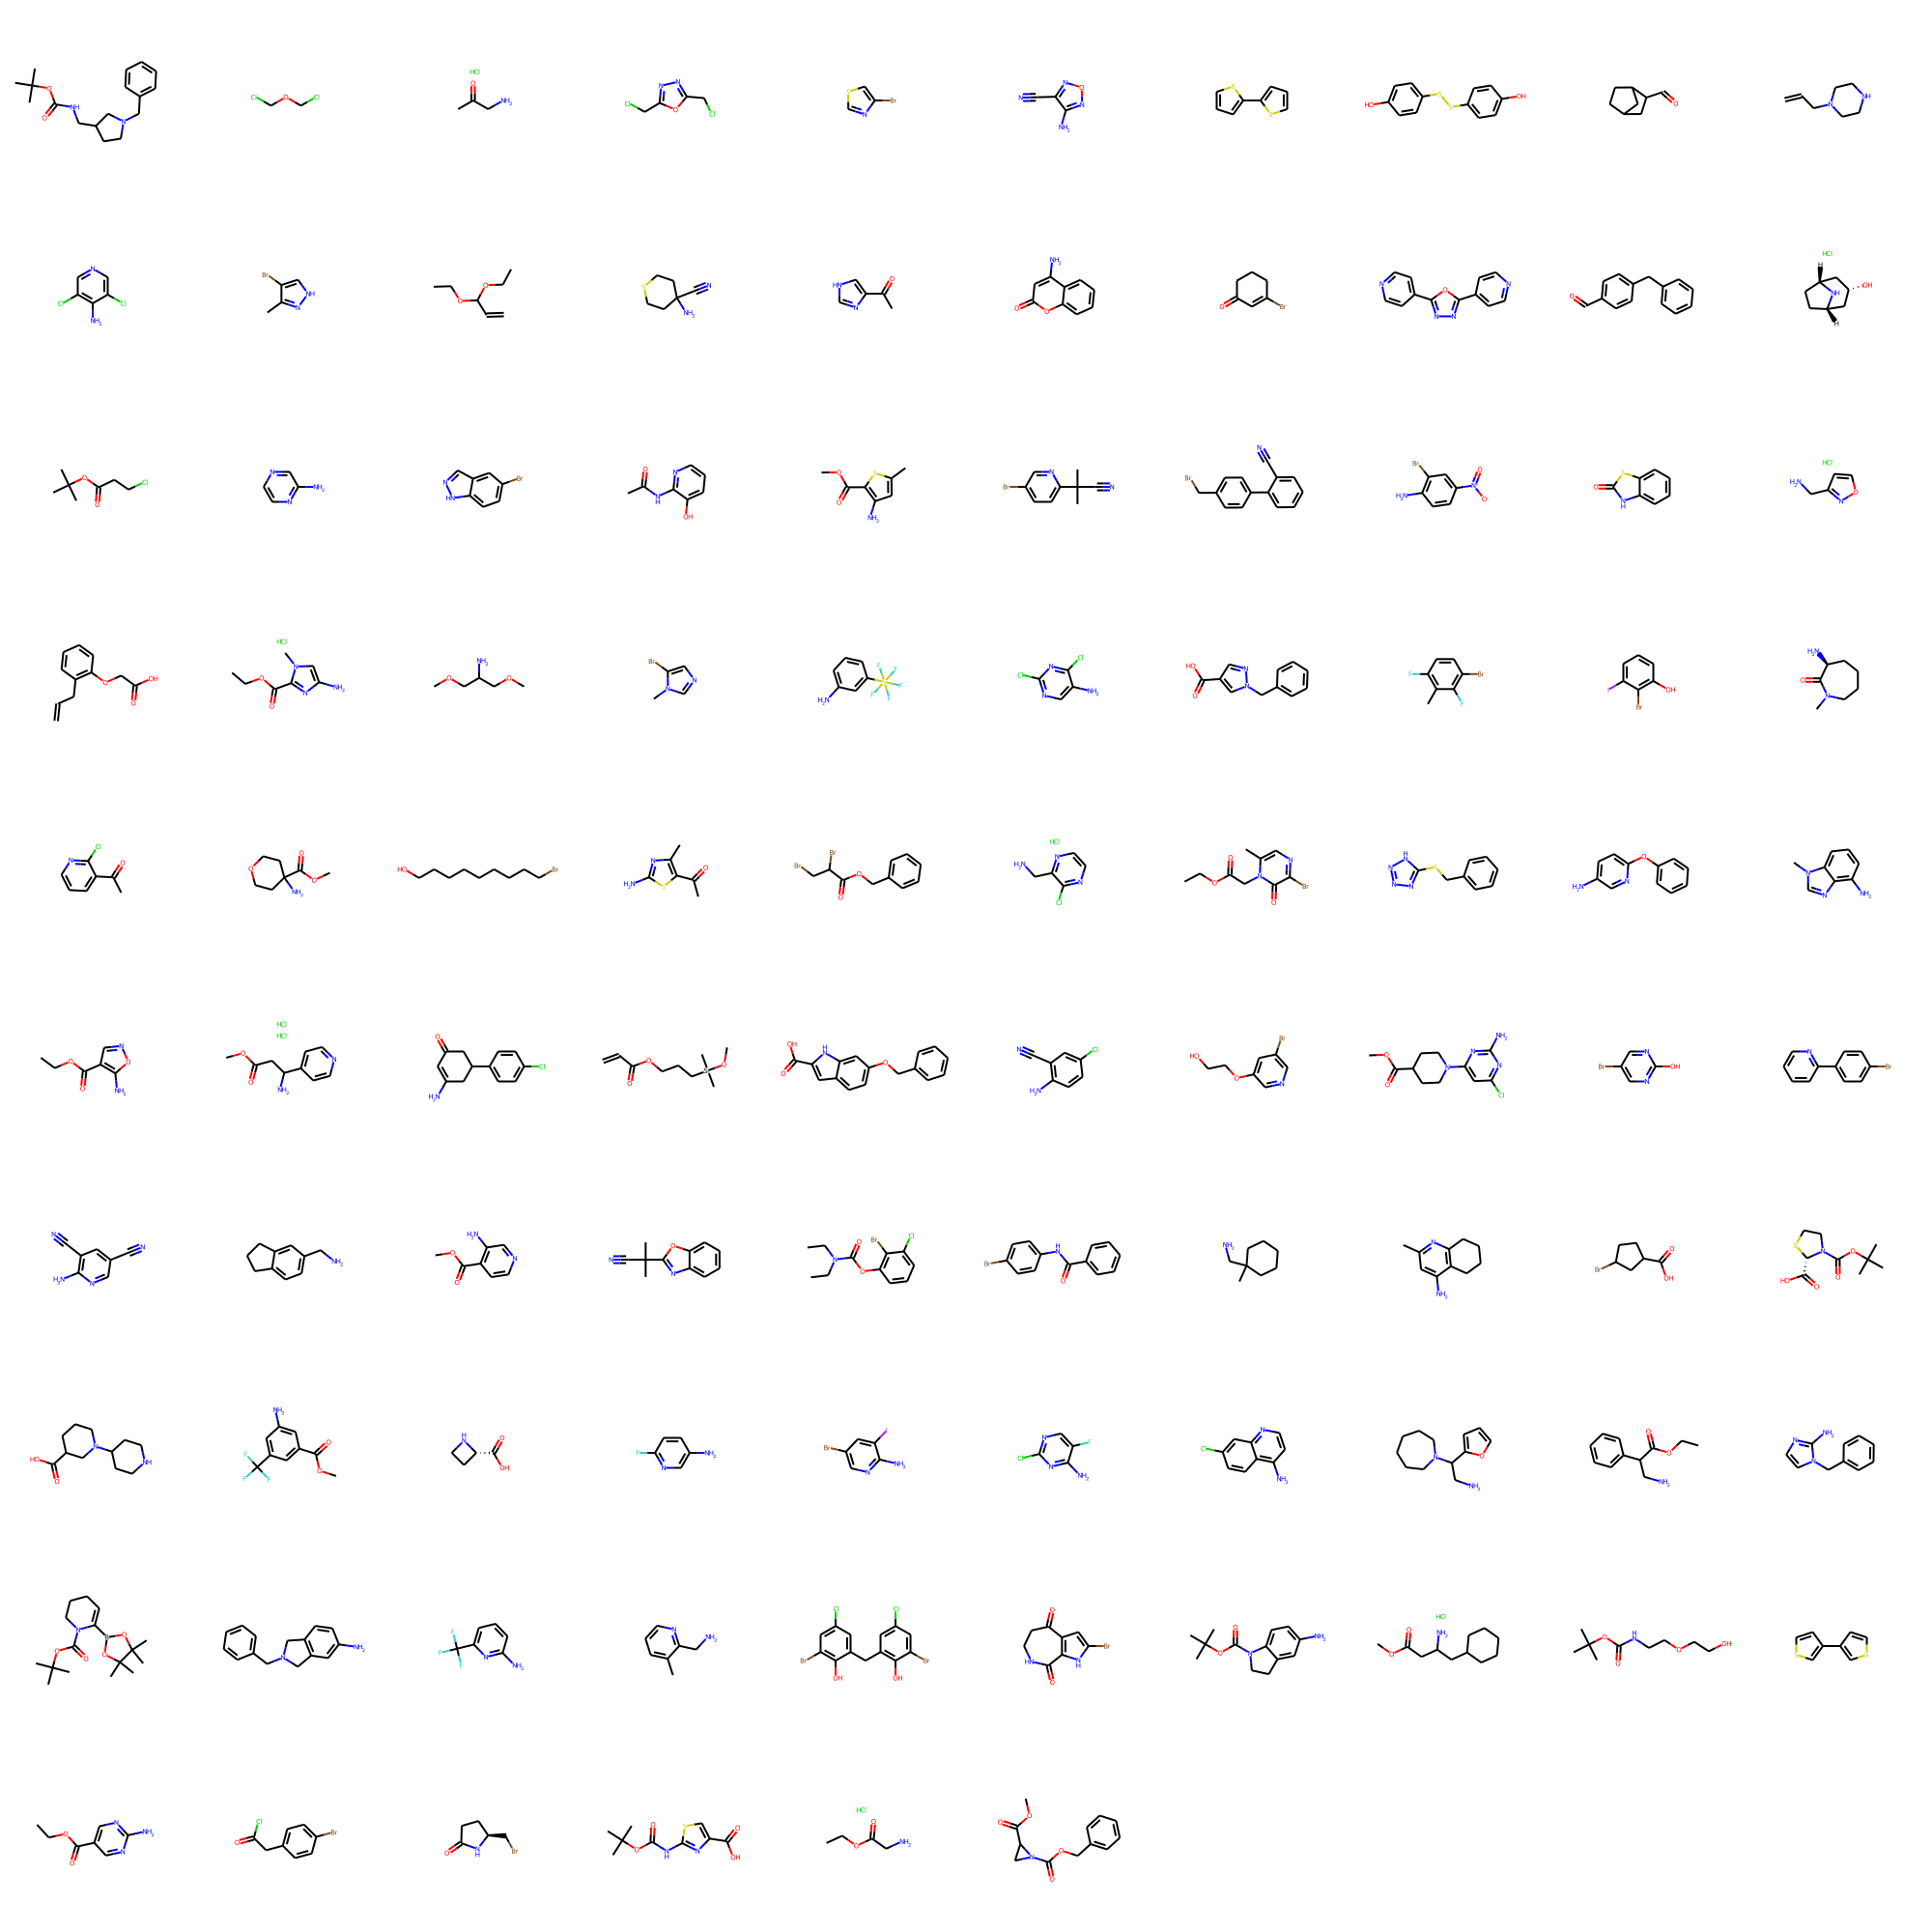
\includegraphics[width=\linewidth]{figs/s979.csv.png}
\end{figure}

\par
Primers for the following 15 notable mutants with broadened substrate binding activity \cite{whitehouse2012p450} were designed with \texttt{mxn} and are being used to assemble the mutants:

\begin{itemize}
  \item GG = E63G/E143G 
  \item GQ = A74G/L188Q 
  \item GVQ = A74G/F87V/L188Q 
  \item IG = F81I/E143G 
  \item II = F162I/M237I 
  \item IV = F81I/E267V 
  \item KT2 = A191T/N239H/I259V/A276T/L353I 
  \item LARV = V26T/R47F/A74G/F87A/L188K 
  \item LF = R47L/Y51F 
  \item LVQ = R47L/F87V/L188Q 
  \item NVN = D168N/A225V/K440N 
  \item QM = V26T/R47F/A74G/F87V/L188K 
  \item QV = L188Q/E267V 
  \item VQ = F87V/L188Q 
  \item VS = F87V/P386S
\end{itemize}

\subsubsection{Primer Design Trial With \texttt{mxn}} \label{mxn}
Primers for the 15 mutants from \cite{whitehouse2012p450} were designed with \texttt{mxn} and ordered. Three generic reverse primers were also designed for the reaction. A trial of the efficacy of these primers to synthesize the mutants LF, VQ and LVQ were carried out with each of the three generic reverse primers. Currently, I have colonies for all reactions and am in the process of prepping the plasmids for sequencing. 
\par
I am waiting on the arrival of another \textit{Agilent QuickChange Multi} kit before I can carry out more reactions.
\par
I am having issues with the quality of sequencing results from Eurofins on wild-type and mutant plasmids, where read length is particularly short despite plasmid DNA submitted was sufficiently pure (> 150 ng / µl, $\frac{260}{280} > 1.9$). Others are having similar issues and I am unsure of how to resolve this.
\par 
DNA work is the major bottle neck in both projects. I will sign an Out of Hours Access form shortly so that I can reduce the time taken for this work as far as possible.

\subsubsection{Data Mining}
\par
Data mining from KEGG has so far yielded around 250,000 P450 sequence-natural ligand pairs for pre-training however with some tweaks this number could be pushed to nearly one million. \cite{biswas2021low} showed that global unsupervised pre-training (all enzyme types) resulted in a model with good performance when transferred to a dataset with only 24 data points. Given the difficultly in fitting simple models to the virtual directed evolution data, I think pretraining a model is essential for the success of this project.
\par
A secondary pre-training dataset - BindingDB (1 million data points) has also been collected. It contains sequences and measured $K_d$, $IC_{50}$ etc. for many drug-like compounds. Secondary pre-training on this dataset will cost little time and effort and may result in a more powerful model, therefore it will be used.
\par 

\subsubsection{Models}
Two similar models are being developed in parallel in this work. Both are deep neural networks that take an input of a protein sequence and a chemical SMILES and embed the combination into a fixed-size representation vector that can be fed to any of a number of output layers to make predictions including but not limited to $K_d$.
\par 
\textbf{Figure \ref{rio diagram}} shows a graph representation of both variants of the model used with neural layer types labelled. The models were written using the \texttt{pytorch} framework. Additional utilities including task specific data loaders have also been constructed.

\begin{figure}[H]
	\caption{\label{rio diagram} Architecture of the two deep neural networks built for this work. \ref{rio-gcn} relies on graph convolutional neural networks for processing chemical inputs, whilst \ref{rio-fp} relies on generating molecular fingerprints ($n$ length binary vector typically $n$ = 1024 or 2048) for processing chemical input. LSTM represents a Long Short Term Memory layer - a type of recurrent layer. MLP represents a Multi-Layer Perceptron - a basic neural network with fully connected layers.}
	\begin{subfigure}{0.49\linewidth}
		\caption{\label{rio-gcn}}
		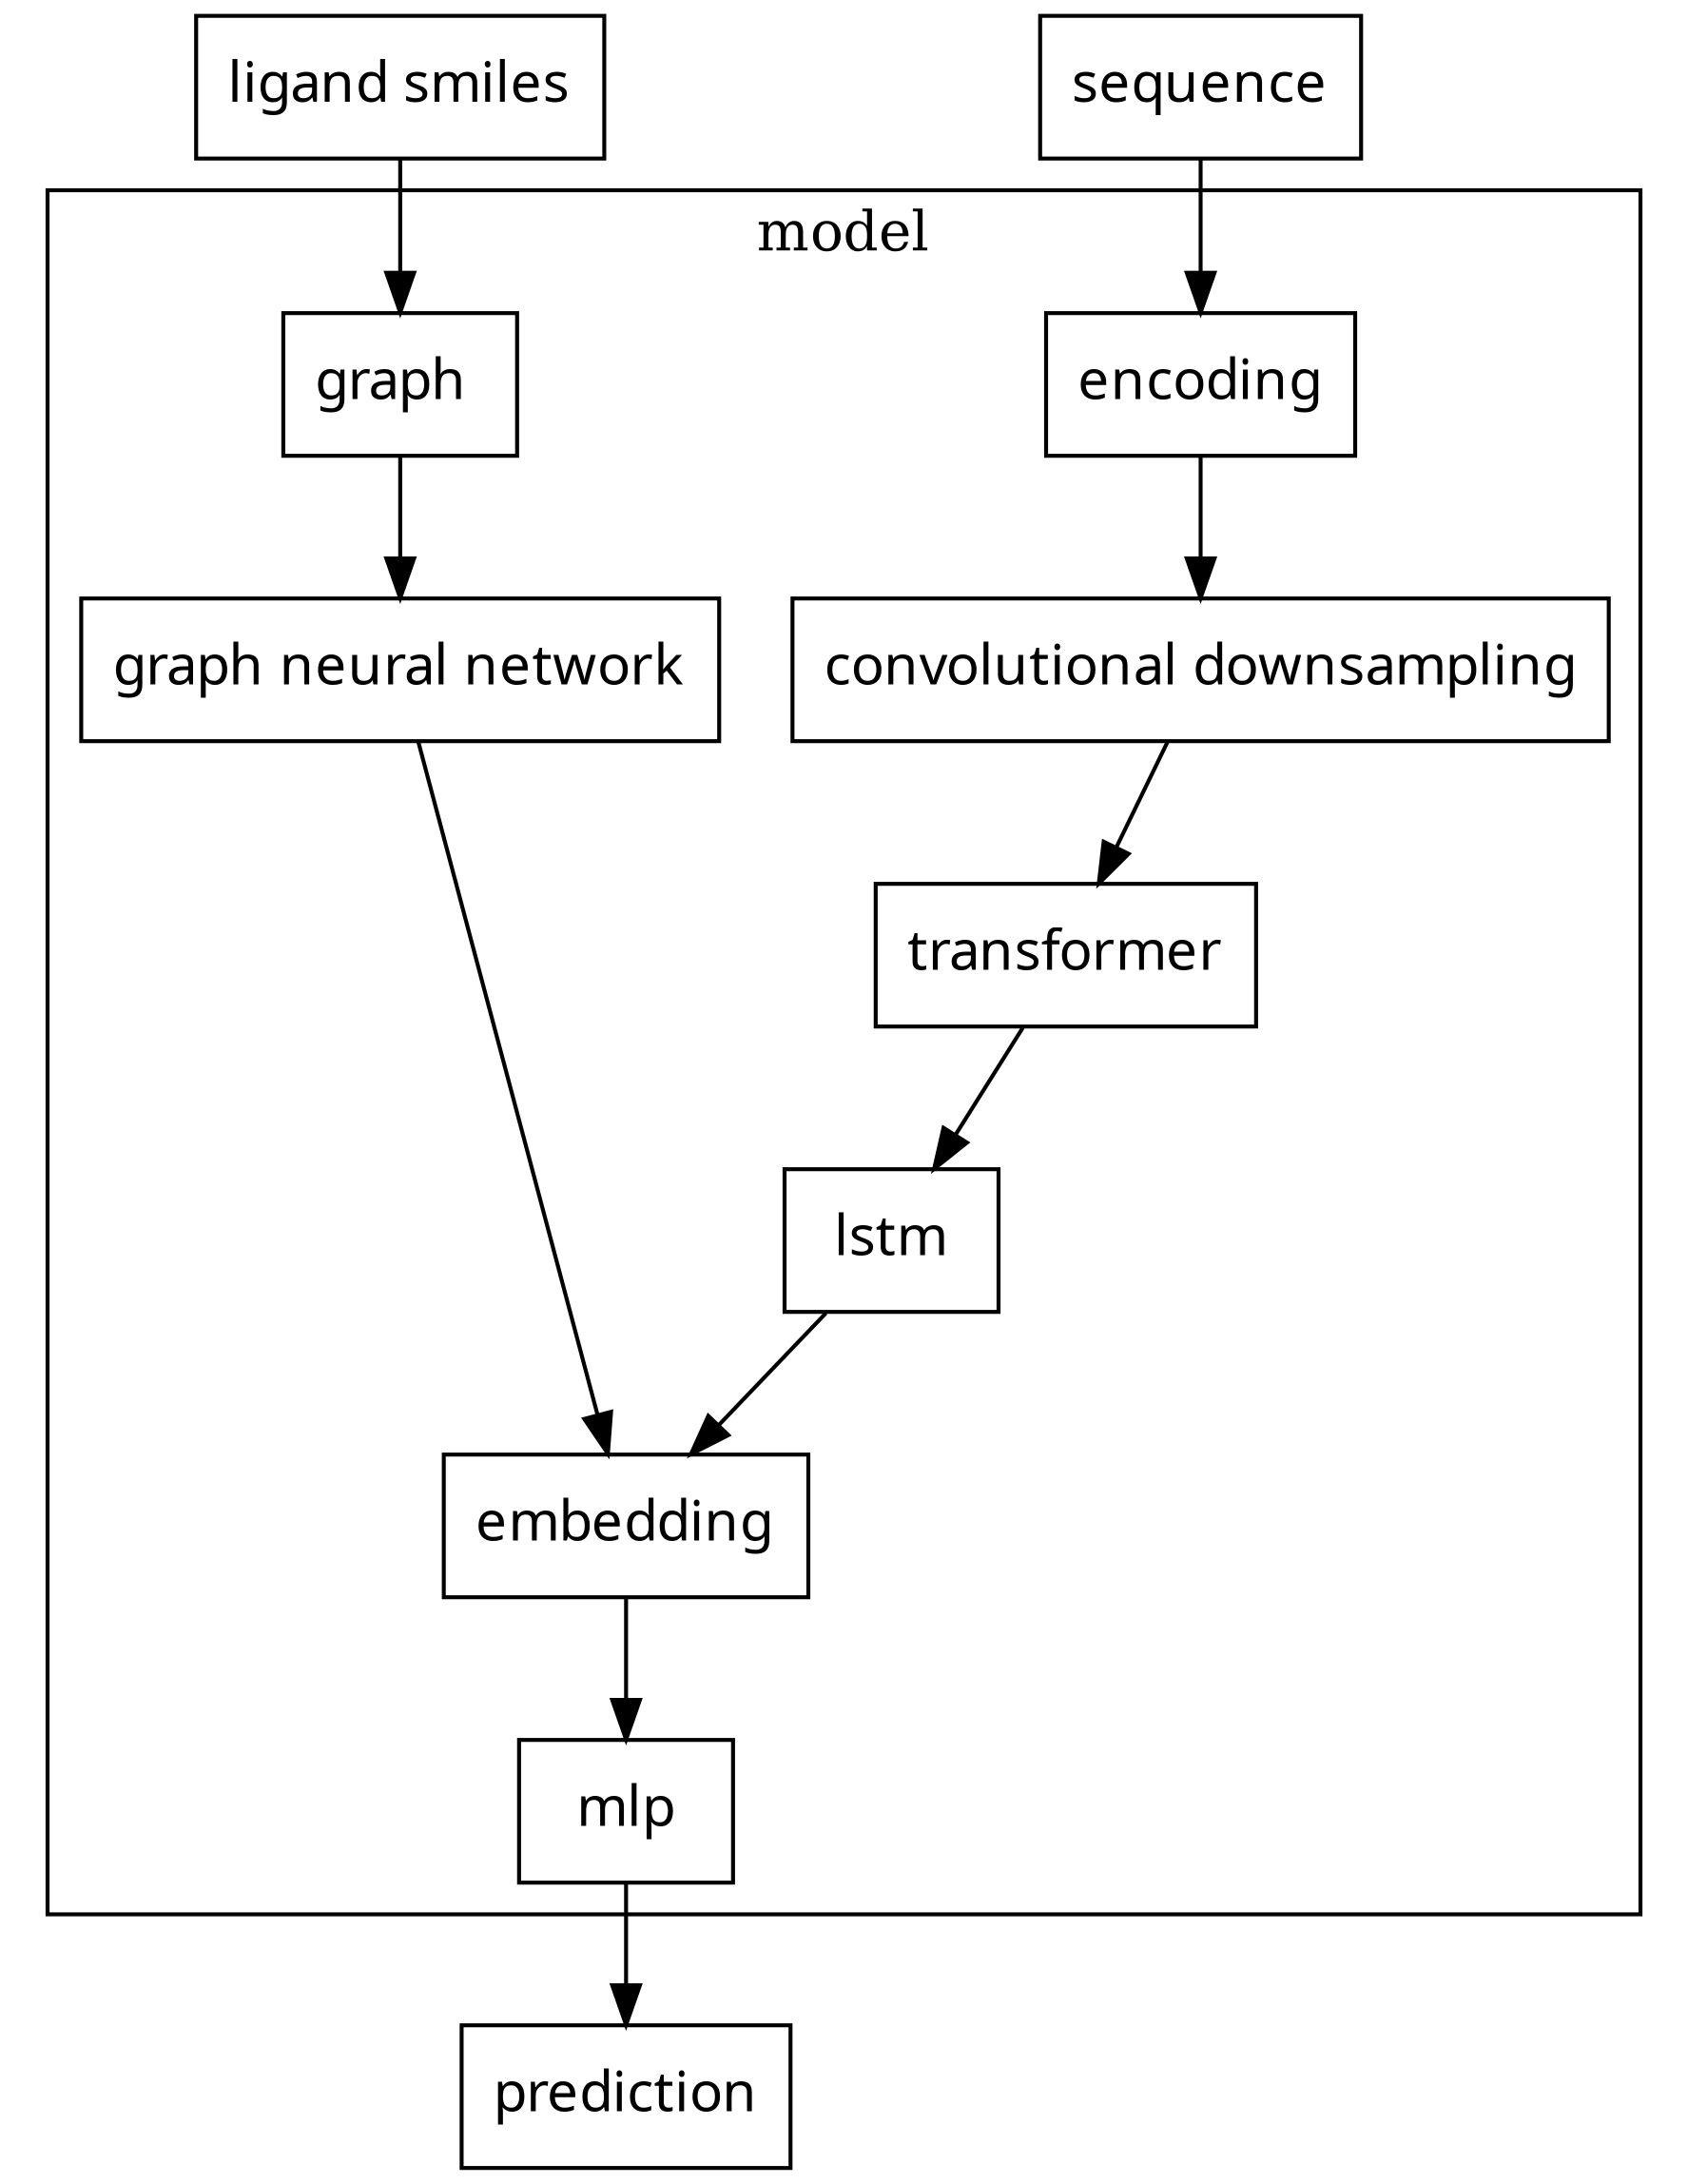
\includegraphics[width=\textwidth]{figs/rio-gcn.png}
	\end{subfigure}
	\begin{subfigure}{0.49\linewidth}
		\caption{\label{rio-fp}}
		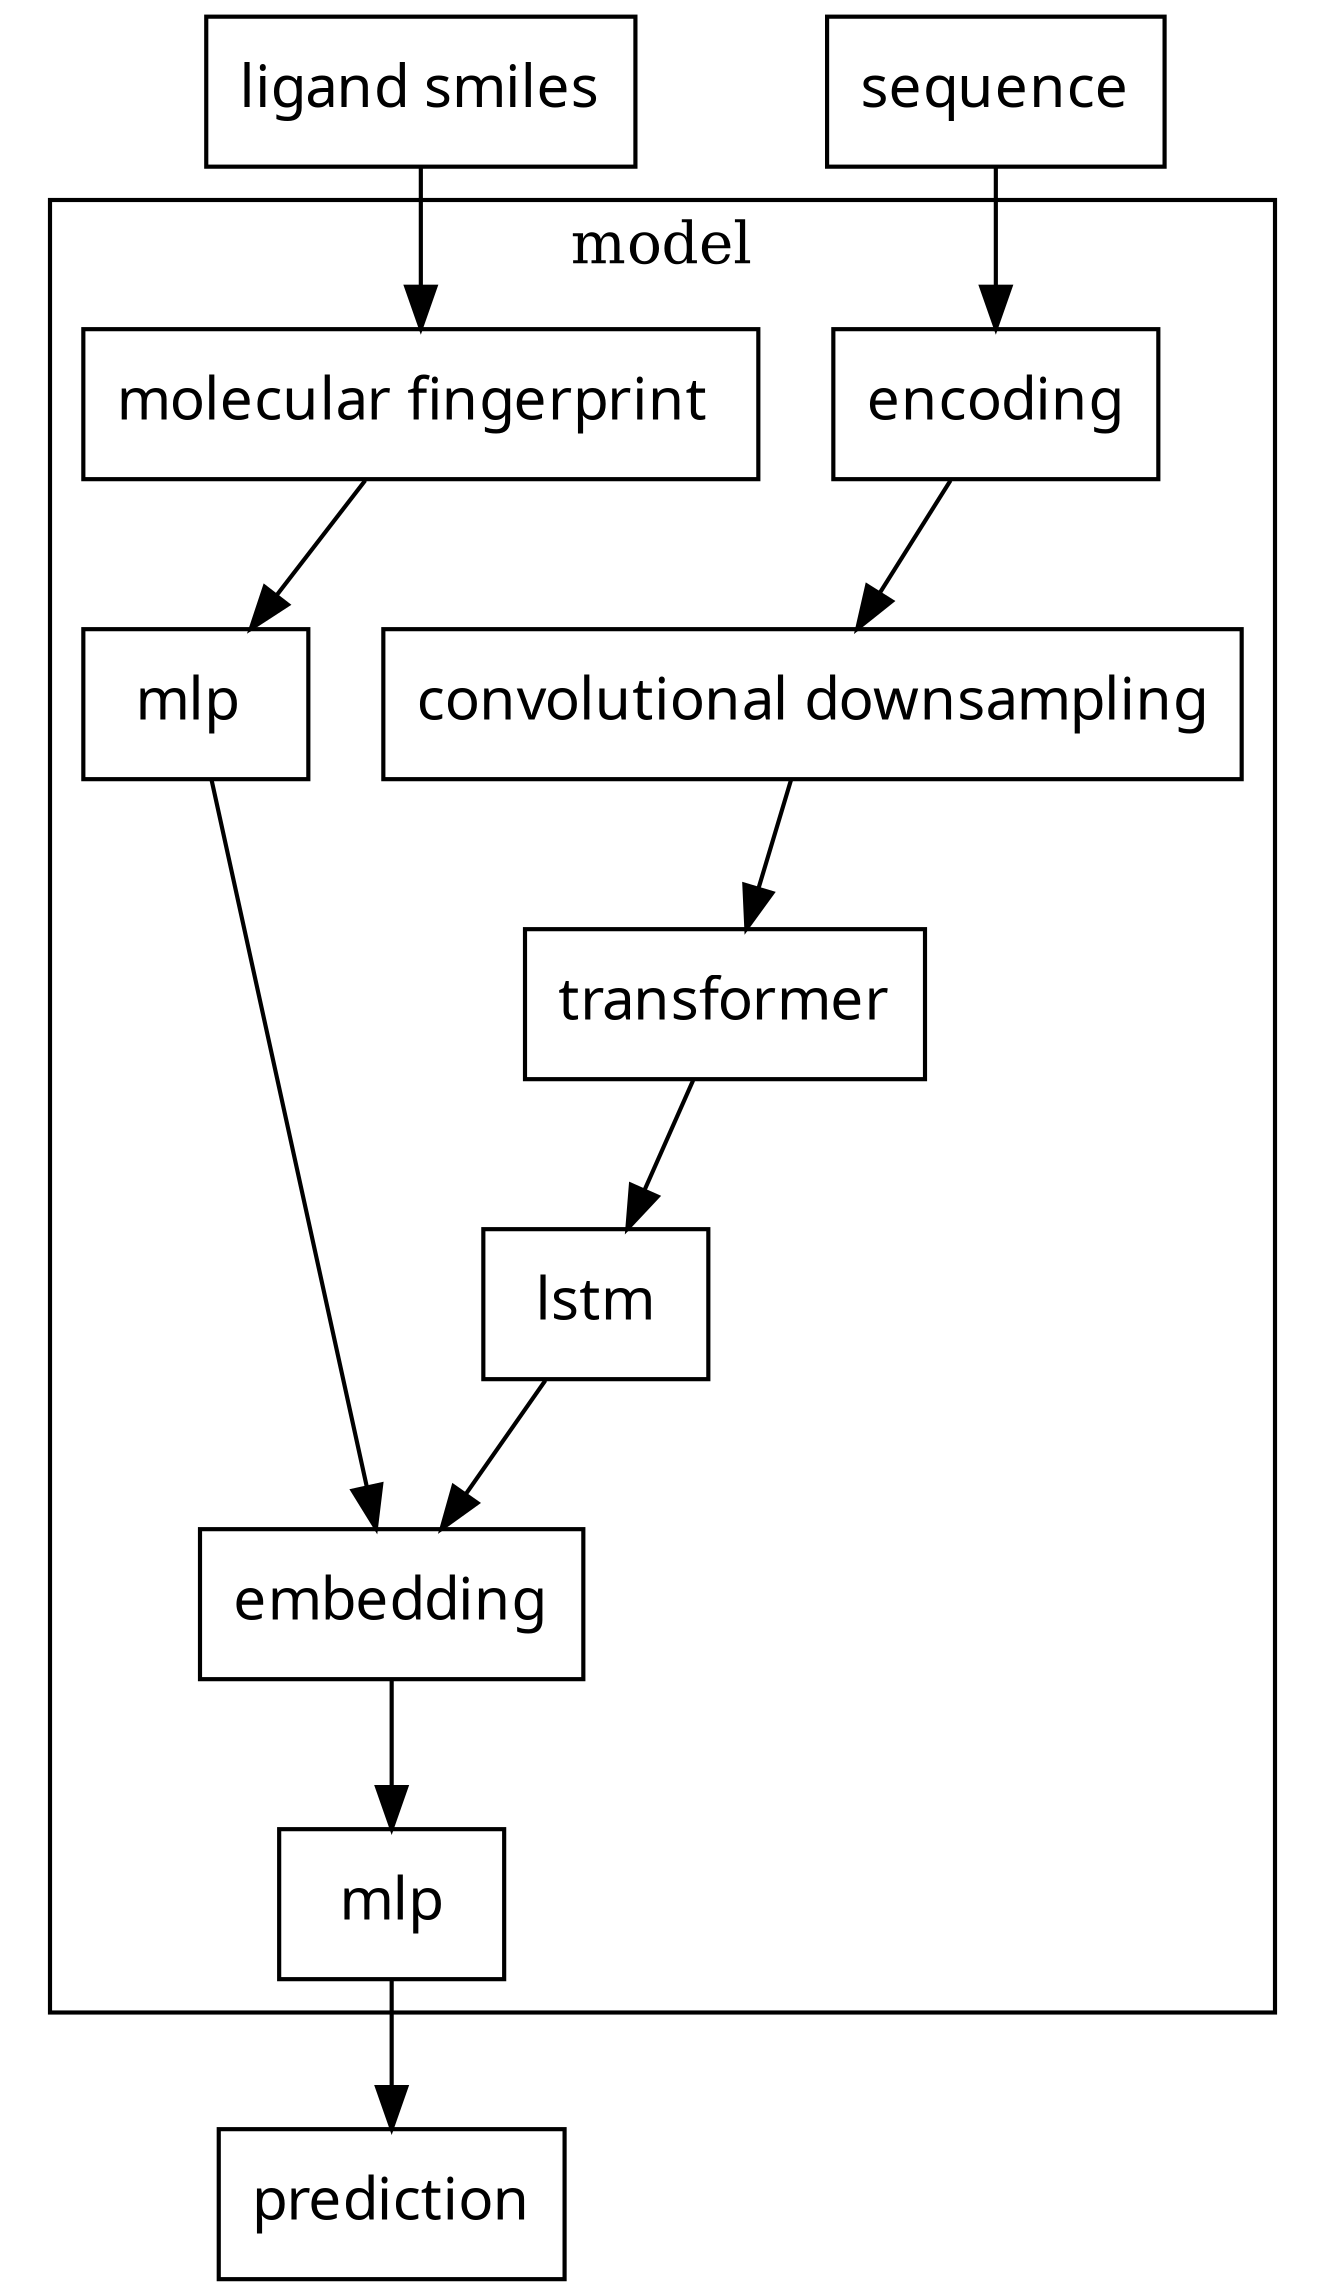
\includegraphics[width=\textwidth]{figs/rio-fp.png}
	\end{subfigure}
\end{figure}
\par 
Both models process protein sequences in the same way:
\begin{enumerate}
	\item \textbf{Encoding:} Amino acids (including ambiguous) are either assigned a one-hot encoding or an engineered feature vector:
		\begin{itemize}
			\item \textbf{One hot encoding:} returns a vector of length $n$ unique amino acids, filled with zeros except at the index assigned to an input amino acid, which is set to 1. For example, if the index for alanine is 0, then \texttt{[1,0,0...]} would be the encoding. The advantage of a one-hot encoding is its simplicity, but its disadvantages include: \textbf{1)} there is no notion of similarity between similar amino acids - for example the encodings for tyrosine and phenylalanine are the same distance from each other as they are from every other amino acid. \textbf{2)} the vectors are fairly information-sparse, which requires more neural parameters to reach a similar result that would be reached by a more dense embedding.
			\item \textbf{Chemical Feature Vector:} returns a vector of length $n$ chemical properties calculated for each amino acid. A set of molecular descriptors are pre-calculated for each amino acid using \texttt{rdkit}, including: \texttt{FormalCharge}, \texttt{NumAliphaticCarbocycles}, \texttt{NumAliphaticHeterocycles}, \texttt{NumAliphaticRings}, \texttt{NumAmideBonds}, \texttt{NumAromaticCarbocycles}, \texttt{NumAromaticHeterocycles}, \texttt{NumAromaticRings}, \texttt{NumBridgeheadAtoms}, \texttt{NumHBA}, \texttt{NumHBD}, \texttt{NumHeteroatoms}, \texttt{NumHeterocycles}, \texttt{NumLipinskiHBA}, \texttt{NumLipinskiHBD}, \texttt{NumRings}, \texttt{NumRotatableBonds}, \texttt{NumSaturatedCarbocycles}, \texttt{NumSaturatedHeterocycles}, \texttt{ExactMolWt}, \texttt{NumSaturatedRings}, \texttt{FractionCSP3}, \texttt{NumSpiroAtoms}. This embedding is fairly straightforward to implement and should offer a richer representation of each amino acid. The issue is how to handle ambiguous amino acids. A potential solution is to take the mean of the chemical properties for the set of amino acids that an ambiguous letter represents.


		\end{itemize}
	\item \textbf{Convolutional Downsampling:} 1D convolutional neural layers compress the sequence whilst preserving spatially invariant features, such as motifs. 
	\item \textbf{Transformer:} An attention-based sequence transduction layer that models the relationships between elements of the input sequence, such as the interplay between different motifs \cite{vaswani2017attention}.
	\item \textbf{Long Short-Term Memory (LSTM):} A recurrent layer that can embed a variable length sequence as a fixed-size vector. It's unclear whether this is necessary since during training, the input sequences are padded to a constant size - therefore the transformer outputs a fixed size sequence. The advantage of this layer is that outside of training, an arbitrary sequence length can be used.
\end{enumerate}
\par 
The models differ in their internal representation of chemical inputs. One uses a traditional molecular fingerprints approach whilst the other uses a more advanced graph neural network architecture.
\par
\begin{itemize}
	\item \textbf{Molecular fingerprints} are fixed-size binary vectors hashed from a molecular structure, originally conceived for chemical similarity searches. Each bit corresponds to the presence or absence of a chemical group or property, with a typical length of 2048. They are simple to implement using \texttt{rdkit} and because of their fixed size, are easily fed to a linear neural layer. They are however, sparse in information compared to more recent methods which perform far better in some tasks. %% ref fp vs graphs
	\item \textbf{Graph Convolutional Neural Networks} are a recent advance in chemical learning which form representations of molecules based on their graph structure.  %% more info & refs
		Asides from their performance, an advantage of graph neural networks is that they can also be used to generate new graphs, which leaves room for extending this model to make graph transformation predictions based on an input molecular graph(s) and an enzyme sequence - prediction of reaction products based on sequence. With sufficient pre-training and active learning, such a model could be a significant advance in enzyme engineering.
\end{itemize}
\par 
In both cases, the sequence and chemical input form a combined representation vector, $z$, which plugs into neural layers that make specific predictions, for example $K_d$. Neural parameters on the input branches are optimized through all training tasks, whilst the final output layers are only optimized on points for which there are data. %%  nah
\par
These mutants are being prepared using Agilent QuickChange Multi kits, which can accommodate up to four mutations per PCR reaction, so all but three of the mutants can be reached in a single reaction. The template sequence used for this work is notably AT-rich and repetitive, which will lead to a certain attrition rate of mutants that are successfully created. It's reasonable to expect to have some usable mutant plasmids by the end of the week starting 3rd May. % expected hit rate?
\par

\subsubsection{Work to do}
Following the availability of expression plasmid, I will express 3 L of each variant heme domain. 3 L expression volumes (half a shaker) is a somewhat risky deviation from the 6 L I have used up to this point, which yields a significant excess of most mutants bar K97C. My ability to express up to 15 mutants then relies on booking eight shakers for 24-36 hour stretches. % expression
\par
Purification is a one step nickel-affinity chromatography column. My last purification was of 3 mutants over three days. Five-six mutants purified per week is possible and up to 15 mutants can be purified over three weeks.
\par
The remains of the FDA library are unlikely to be sufficient for screening more than five more mutants, it is past its expiry date and all vials have been used for titrations in the past, so contamination is likely. Therefore, I think it is important that I order a set of 96 herbicide-like compounds from MolPort to cover the remainder of my screening operation. %%%% calc vol & price estimate
\par
With an average compound consumption of 12 µl (10 mM in DMSO) per mutant, plus controls (typically one control per 3 mutants screened) I need at least 240µl of each compound to screen all 15 mutants at 10 mM or 24 µl at 100 mM. 96 compounds is a practical number to screen and the compounds must be a representative sample of the chemical space surrounding herbicides. 
\par
I need to re-run the MolPort compound selection program with a more up-to-date copy of the MolPort library and with an additional filter for herbicide likeness based on Tanimoto similarity to one or more herbicides.
%%%%%%%%%%%% molport program
\par
With a lead time of one month, the compounds would arrive in time for the mutants in construction to be purified. %% time estimate 
\par 
In this case, the final round of screening with all available mutants against the 96 compounds would likely start and finish in June. 
\par 
Up until the availability of all screening data, the model can be pre-trained on both datasets. Success of initial, unsupervised pre-training on KEGG is difficult to quantify directly but would become apparent on transfer to the supervised BindingDB task. I have access to sufficient computational resources to train the model.
\par 
Re-training the model on the screening dataset will not take long, given its small size (minutes). After this, the model can be used to design new BM3 variants by guiding a sequence optimizer towards a sequence with a low estimated $K_d$ towards mesotrione. The existing genetic algorithm used in the Virtual Directed Evolution project is a suitable optimizer in this case and should converge on a set of mutants in minutes after deployment.
\par
For practical assembly of proposed mutants, the genetic algorithm should be restrained by $n$ mutations from existing template sequences, where $n$ is four-eight depending on time constraints.
\par
Primers for six-eight of these mutants can be designed with \texttt{mxn} automatically and the mutants can be assembled from existing full-length protein templates using Agilent QuickChange Multi mutagenesis kits at up to four mutations at a time. % timeline?
\par 
Following expression vector assembly I can express the mutants in 3L batches as with Virtual Directed Evolution project, which requires eight 24 hour shaker slots. Purification can be done over the course of two weeks and testing another one-two weeks, reaching the end condition for this project.
\par 
\textbf{Figure \ref{rioG}} shows a dependency graph of the remainder of the project. A Gantt chart for the remaining tasks in this work is in \ref{rio gantt}.


%%%%%% graph fig %%%%%%%%%%%%%
\begin{figure}[H]
	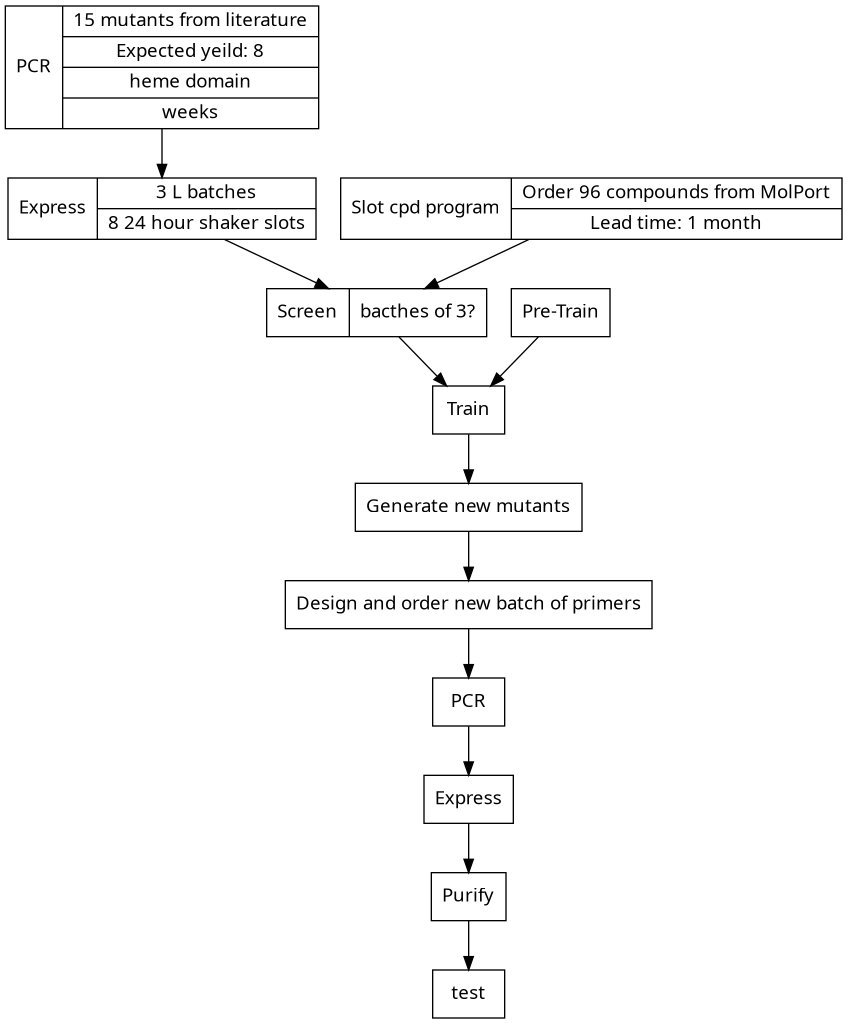
\includegraphics[width=\textwidth]{figs/rioG.png}
	\caption{\label{rioG} Dependency graph for remainder of the AI-based design project}
\end{figure}


%%%%%%%%%%%%%%%%%%% ganntt chart
\newgeometry{vmargin = 1cm}
\begin{landscape}
	\subsection{Gantt Chart} \label{rio gantt}
	\centering
	\fontsize{6pt}{8pt}
\begin{ganttchart}[time slot format=isodate, x unit = 1.8mm, vgrid, hgrid]{2021-05-17}{2021-09-18}{week}
	\gantttitlecalendar{month = name, week=3} \\
	\ganttbar{DNA Work}{2021-05-17}{2021-06-09} \\
	\ganttbar{Compound Selection}{2021-05-17}{2021-05-26} \\
	\ganttbar{Expression}{2021-05-26}{2021-06-25} \\
	\ganttbar{Purification}{2021-06-18}{2021-07-03} \\
	\ganttbar{Screening}{2021-06-20}{2021-07-17} \\
	\ganttbar{Pre-Training}{2021-07-03}{2021-07-17} \\
	\ganttbar{Training}{2021-07-17}{2021-07-24} \\
	\ganttbar{Mutant Generation}{2021-07-24}{2021-07-31} \\
	\ganttbar{Primer Design}{2021-07-31}{2021-08-02} \\
	\ganttbar{DNA work}{2021-08-09}{2021-08-21} \\
	\ganttbar{Expression}{2021-08-21}{2021-09-04} \\
	\ganttbar{Purification}{2021-08-26}{2021-09-08} \\
	\ganttbar{Validation}{2021-09-03}{2021-09-12} \\
\end{ganttchart}
\end{landscape}
\restoregeometry
%%%%%%%%%%%%%%5

\section{Lab Work} 
Both the virtual directed evolution and the AI-based design work have significantly overlapping lab work requirements and therefore some tasks can be batched together.
\begin{table}[H]
	\centering
	\begin{tabular}{lcr}
		\textbf{Task} & \textbf{Virtual Directed Evolution} & \textbf{AI-based Design} \\
		\hline
		DNA work & 8 mutants & < 15 mutants; 8 mutants \\
		Expression & 8 mutants & < 15 mutants; 8 mutants \\
		Protein Purification & 8 mutants & < 15 mutants; 8 mutants \\
		Screening & & < 15 mutants \\
		Binding Titrations with Mesotrione & 8 mutants & 8 mutants \\
		NADPH consumption with Mesotrione & 8 mutants & 8 mutants\\
		Product formation indication with LCMS & 8 mutants & 8 mutants\\
	\end{tabular}
\end{table}
\par
\subsection{DNA work}
The current bottle neck for both projects is DNA work, which is inherently time-consuming and error-prone. A mitigation to the time consuming nature taken is use of \textit{Agilent QuickChange Multi} mutagenesis, which allows up to four mutations to be made at a time. Another mitigation I will take is working out of hours, which can save a significant amount of time. A problem I currently face is the quality of sequencing results from the supplier \textit{Eurofins}, where the reads are particularly short and noisy for samples sent that adhere to their submission requirements. I am unsure on how to approach this issue in a cost-effective manner.
\par 
Current work is in the DNA synthesis of the < 15 screening mutants for the AI-based design project. A new \textit{Agilent QuickChange Multi} mutagenesis kit has just arrived. This week I will start to finish the construction of the screening mutants. Synthesis of the 8 validation mutants from the virtual directed evolution experiments will begin in late May, once I have re-run the experiment with patches for the issues mentioned in section \ref{vde-todo}.
\par 
\subsection{Protein Expression}
Mutant expression in both projects is straightforward, with growth in auto-induction Terrific Broth over 24-48 hours at 25°C after an initial 3-4 hours at 37°C. Use of auto-induction broth mitigates the risk of phage contamination over growth, as well as reducing physical work required compared to non-auto-induction media.

\begin{table}[H]
	\begin{tabular}{lccc}
		\textbf{Batch} & \textbf{Vol per mutant} & \textbf{Total Volume} & \textbf{Number of Shakers} \\
		\hline
		< 15 screening mutants & 3 L & 45 L & 5 \\
		8 validation mutants & 3L & 24 L & 4 \\
		8 validation mutants & 3L & 24 L & 4 \\
		\hline
		\textbf{Total} & & 96 L & 13 \\
	\end{tabular}
\end{table}

\subsection{Protein Purification}
For all proteins to be expressed in the project, purification is:
\begin{enumerate}
	\item Lyse pellet with sonication, centrifuge and retain supernatant
	\item Remove additional particulates and unstable protein with a 30\% Ammonium Sulfate cut and centrifuge, retaining supernatant
	\item Extract His-Tagged target protein with Nickel-Affinity chromatography
	\item Dialyse into 100 mM KPi (pH 7)
	\item Concentrate protein to around 500 - 900 µM and flash freeze.
\end{enumerate}
Recently I staggered the start of three purifications by 30 minutes, which was manageable and the purification for all was finished within three days of start. Six purifications in a week is feasible, potentially more depending on how efficiently I manage the tasks. 
\par
% timeline

\subsection{Screening}
I can comfortably screen three mutants against 96 compounds per day and the Cai lab member who I coordinate for using the \textit{Echo} often works on weekends, so weekend screening is feasible. It's unclear how much data is needed to make AI-based enzyme design work, so I'm opting for as much as possible. This maximises the chances of success and also maximises the re usability of the model, which is a high priority.
\par
I've planned the expression and purification of up to 15 additional mutants; to screen all 20 against the proposed compound library requires 7 days of screening. 
\par
I currently have five purified BM3 mutants in stock and some FDA compounds left, perhaps enough to screen five or so mutants. One contingency plan on the inability to secure a compound library is to screen the remaining FDA compounds, stretching them as far as possible. I need to inventory the compounds I have to know how far they will stretch. %% option - FDA screen, how much protein? enough to do both?
\par

\subsection{Validation}
Validation of new mutants will be against mesotrione only using standard techniques. For each mutant, I need to know $K_d$, $K_M$, $K_{cat}$ and an indication of product formation. The techniques are:
\begin{itemize}
	\item $K_d$: UV-Vis spectroscopy titrations with mesotrione. Each titration can be done in around 30 minutes
	\item $K_M$ and $K_{cat}$: UV-Vis spectroscopy based NADPH consumption assay with mesotrione 
	\item \textbf{Indication of product formation: } LCMS of bio transformation reactions with mesotrione. I will need to set out a method for this, but there are experts in this around.
\end{itemize}


\newgeometry{vmargin=1cm}
\begin{landscape}
	\subsection{Gantt Chart - All Remaining Work} \label{gantt all}
	\centering
	\fontsize{6pt}{8pt}
\begin{ganttchart}[time slot format=isodate, y unit chart = 5mm, x unit = 1.8mm, vgrid, hgrid]{2021-05-17}{2021-09-18}{week}
	\gantttitlecalendar{month = name, week=3} \\
	\ganttbar{\textbf{VDE:} VDE}{2021-05-17}{2021-05-25} \\
	\ganttbar{\textbf{VDE:} Primer Design}{2021-05-25}{2021-05-26} \\
	\ganttbar{\textbf{VDE:} Primer Shipping}{2021-05-26}{2021-06-03} \\
	\ganttbar{\textbf{VDE:} DNA work}{2021-06-03}{2021-06-17} \\
	\ganttbar{\textbf{VDE:} Expression}{2021-06-11}{2021-06-25} \\
	\ganttbar{\textbf{VDE:} Purification}{2021-06-18}{2021-07-03} \\
	\ganttbar{\textbf{VDE:} Validation}{2021-07-03}{2021-07-10} \\
	\\
	%%%%%%%%%%%
	\ganttbar{\textbf{AI: }DNA Work}{2021-05-17}{2021-06-09} \\
	\ganttbar{\textbf{AI: }Compound Selection}{2021-05-17}{2021-05-26} \\
	\ganttbar{\textbf{AI: }Expression}{2021-05-26}{2021-06-25} \\
	\ganttbar{\textbf{AI: }Purification}{2021-06-18}{2021-07-03} \\
	\ganttbar{\textbf{AI: }Screening}{2021-06-20}{2021-07-17} \\
	\ganttbar{\textbf{AI: }Pre-Training}{2021-07-03}{2021-07-17} \\
	\ganttbar{\textbf{AI: }Training}{2021-07-17}{2021-07-24} \\
	\ganttbar{\textbf{AI: }Mutant Generation}{2021-07-24}{2021-07-31} \\
	\ganttbar{\textbf{AI: }Primer Design}{2021-07-31}{2021-08-02} \\
	\ganttbar{\textbf{AI: }DNA work}{2021-08-09}{2021-08-21} \\
	\ganttbar{\textbf{AI: }Expression}{2021-08-21}{2021-09-04} \\
	\ganttbar{\textbf{AI: }Purification}{2021-08-26}{2021-09-08} \\
	\ganttbar{\textbf{AI: }Validation}{2021-09-03}{2021-09-12} \\
\end{ganttchart}
\end{landscape}
\restoregeometry

\section{Scenarios and Contingencies} \label{contingencies}

\subsection{No Extension}
The strategy laid out in the Gantt charts assumes no funded extension though I will almost certainly need a submission deadline extension to allow time for writing. The schedule is tight and has little room for error. Tasks that can be reduced are:
\begin{itemize}
	\item \textbf{Screening - mutants:} Time can be saved by screening fewer mutants. The subset of the original selection should contain mutants with as varied substrate scope as possible. This can be done by finding the substrate scope of the mutant panel from \cite{whitehouse2012p450} and either selecting based on judgement or by re-implementing MaxMin sampling on the substrate scope of the set. Alternatively MaxMin sampling can be applier to the physical-chemical properties of the active site of each mutant fairly easily. The selection may be limited by unsuccessful DNA syntheses.
	\item \textbf{Screening - compounds:} If availability of the proposed compound library is a time-limiting factor, then the FDA compounds can be screened instead. This strategy may be combined with a reduced screening set.
\end{itemize}

\subsection{Unfunded Deadline Extension}
In this case, lab work remains more or less the same, only some time that would otherwise be spent writing will be freed up. 

\subsection{Funded Deadline Extension}
In this case, I would like to use as little of the extra time as possible so that I can start full time work. In this case I will reduce the project as necessary to finish in October. Funding will make the necessary DNA work far more feasible, since I'm currently constrained by budget with respect to DNA synthesis and sequencing.

\subsection{No Compound Library}
In the event that I can not secure a compound library, I will have to screen as many of the mutants as I can against the remaining FDA compounds. In this case the screening operation will be limited by the availability of the remaining FDA compounds. I can take an inventory of all remaining compounds and pool duplicates, then I can accurately estimate how many mutants I can screen. I currently estimate 5-10. 

\subsection{Failed DNA Synthesis of Screening Mutants}
In the event that DNA synthesis of some or all of the screening mutants fails or is not possible, then I will have to capture as much screening data with what mutants I do have. I can increase the number of compounds screened against each mutant and scour for BM3 mutant plasmids in the Munro Lab. 
\par

\section{Thesis Layout} \label{thesis layout}
I aim to structure my thesis in alternative/journal-style submission format with two chapters and several supplementary sections. Neil Burton agreed that given the circumstances, two chapters is acceptable. % thesis format
\par 
I aim to fill the supplementary sections with my software development for tools that I rely on for this work, and details of assay development.

\par
\par

{\large\textbf{Engineering a P450 BM3 mutant for herbicide detoxification}}
\\
\begin{enumerate}
	\item \textbf{Virtual directed evolution}
		\begin{itemize}
			\item \textbf{Introduction:} 
				\begin{itemize}
					\item Herbicide resistance and P450s in herbicide metabolism
					\item P450 engineering for herbicide resistance
					\item BM3 engineering and experimental techniques
					\item Directed Evolution 
					\item Protein structure prediction 
					\item Docking 
					\item Project aims: virtual directed evolution
				\end{itemize}
			\item \textbf{Methods:}
				\begin{itemize}
					\item \texttt{enz}
					\item genetic algorithm and virtual directed evolution
					\item DNA work and \texttt{mxn}
					\item expression and purification 
					\item validation
				\end{itemize}
			\item \textbf{Results:}
				\begin{itemize}
					\item virtual directed evolution analysis - summary stats, fitness landscape (t-SNE), Pareto front, diversity selection, pymol visualised mutant selection
					\item validation results
					\item predicted results vs actual
				\end{itemize}
			\item \textbf{Discussion:}
				\begin{itemize}
					\item Critique of virtual directed evolution technique used - how well do predicted results match lab results.
					\item Future Improvements to \texttt{enz}
				\end{itemize}
		\end{itemize}
	\item \textbf{AI-based design}
		\begin{itemize}
			\item \textbf{Introduction:}
				\begin{itemize}
					\item Herbicide resistance and P450s in herbicide metabolism
					\item P450 engineering for herbicide resistance
					\item BM3 engineering and experimental techniques
					\item Machine learning-guided protein engineering 
					\item Machine learning techniques: chemical learning, sequence learning, transfer learning
					\item 
					\item Project aims: general AI-based BM3 design
				\end{itemize}
			\item \textbf{Methods:}
				\begin{itemize}
					\item Plate assay development 
					\item mutant selection 
					\item compound selection 
					\item screening 
					\item model architecture and training
					\item sequence generation
					\item DNA work
					\item expression and purification 
					\item validation
				\end{itemize}
			\item \textbf{Results:}
				\item Screening results and data quality
				\item model training and accuracy
				\item Sequence generation - plot fitness landscape, Pareto front 
				\item Validation - 
			\item \textbf{Discussion:}
				\begin{itemize}
					\item Validation - expected vs actual results
					\item screening data quality
					\item model accuracy
					\item strength and drawbacks of techniques 
					\item proposed improvements to model accuracy - e.g. more screening data, different architecture 
					\item future work: chemial transform learning and active learning - robot scientist
				\end{itemize}
		\end{itemize}
\end{enumerate}

\par
{\large \textbf{Supplementary}}
\begin{itemize}
	\item \textbf{Assay Development}
	\item \textbf{\texttt{enz} Development}
	\item \textbf{Other software tool development} 
		\begin{itemize}
			\item \texttt{mxn} - DNA design tool
			\item \texttt{echo} - echo experiment design tool
			\item \texttt{plates} - plate assay analysis tool
			\item \texttt{cpd} - compound selection tool
		\end{itemize}
\end{itemize}
\par
\printbibliography

\end{document}
